\chapter{Teil 1 Mechanik}
\section{Einleitung}
\section{Aufgabenstellung}
\subsection{Zielsetzung}
\subsection{Problematik}
\newpage
\section{Konzepte} 



\subsection{Variante 1} 
\subsubsection{Übersicht der Prozessschritte}
\begin{itemize}
\item[1] Füllen des Futtermagazins
\item[2] Führen zur Schneidplatte
\item[3] Schnitt
\item[4] Pressen
\item[5] Entsorgen
\item[6] Füttern
\end{itemize}

\subsubsection{Füllen des Futtermagazins}

Im den folgenden Bildern wird mithilfe einer Lego-Darstellung gezeigt, wie das Magazin aus verschiedenen Blickwinkeln befüllt aussieht. Hier muss man beachten das die vom Hersteller zu öffneten Seite in Richtung des Schneidewerks zeigt (die schmale Seite mit der Einkerbung). Siehe Abbildungen: \ref{Magazin Vorne}, \ref{Magazin Seitlich}, \ref{Magazin Oben}, 

\begin{figure}[H]
\begin{center}
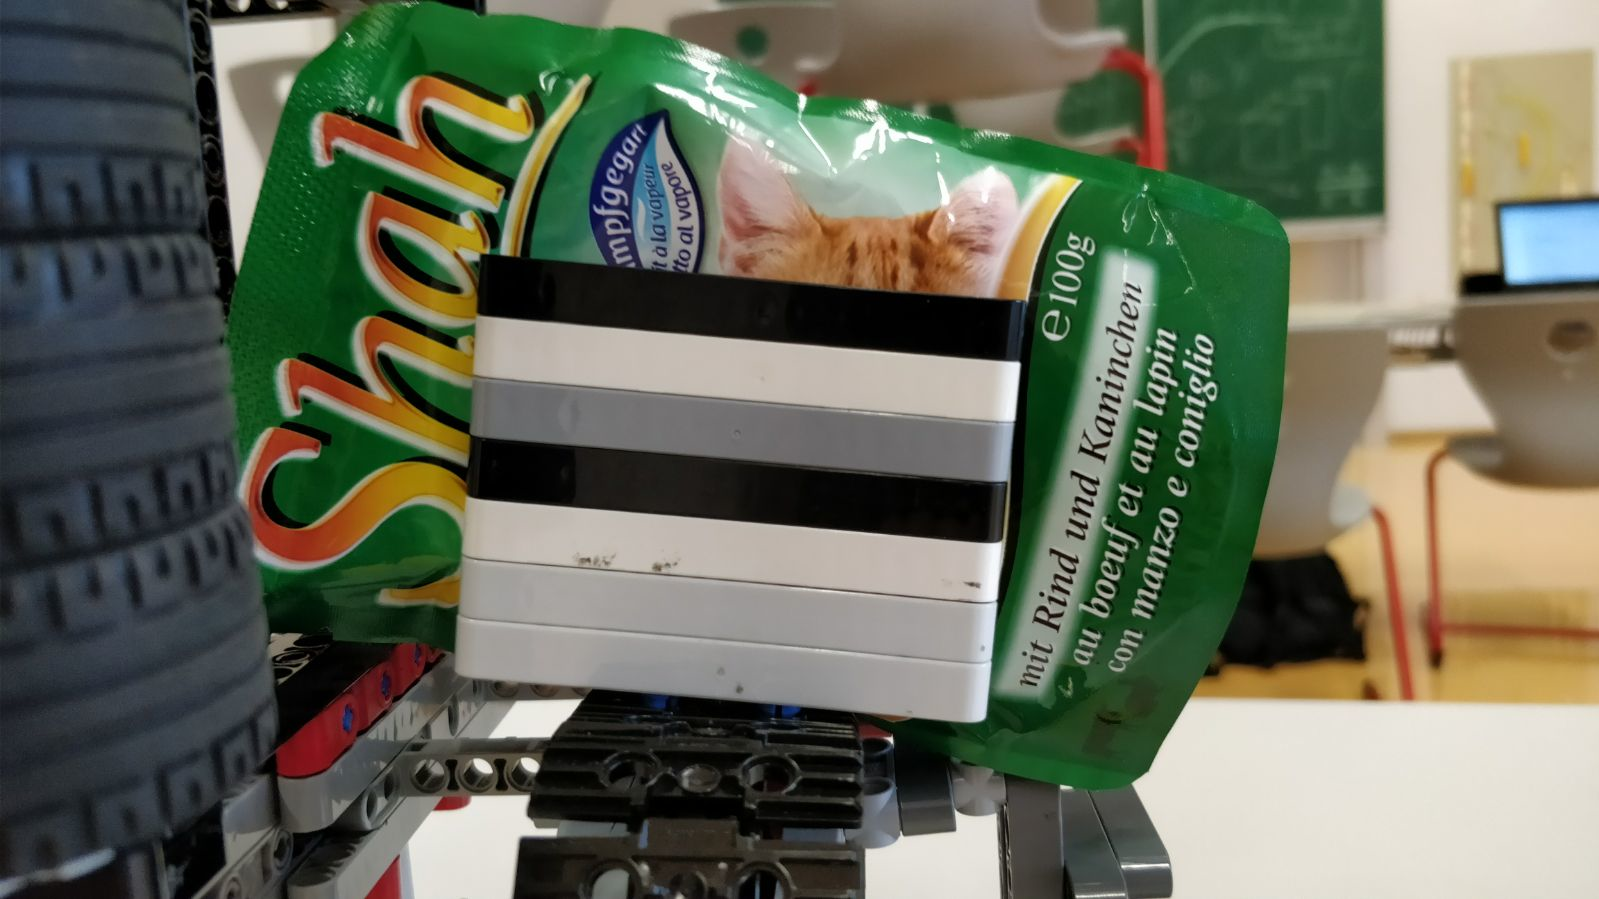
\includegraphics[width=13cm]{Bilder/Ablauf_1_png/Magazin_Vorne.png}
\caption{Magazin Vorne}
\label{Magazin Vorne}
\end{center}
\end{figure}

\begin{figure}[H]
\begin{center}
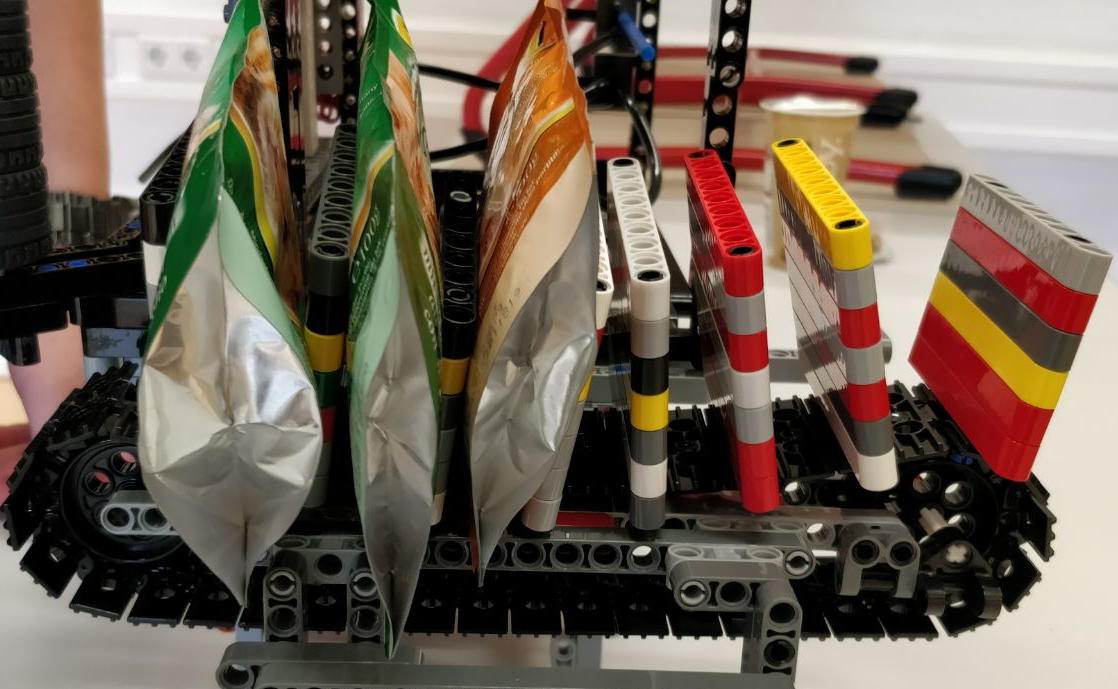
\includegraphics[width=13cm]{Bilder/Ablauf_1_png/Magazin_Seitlich.png}
\caption{Magazin Seitlich}
\label{Magazin Seitlich}
\end{center}
\end{figure}

\begin{figure}[H]
\begin{center}
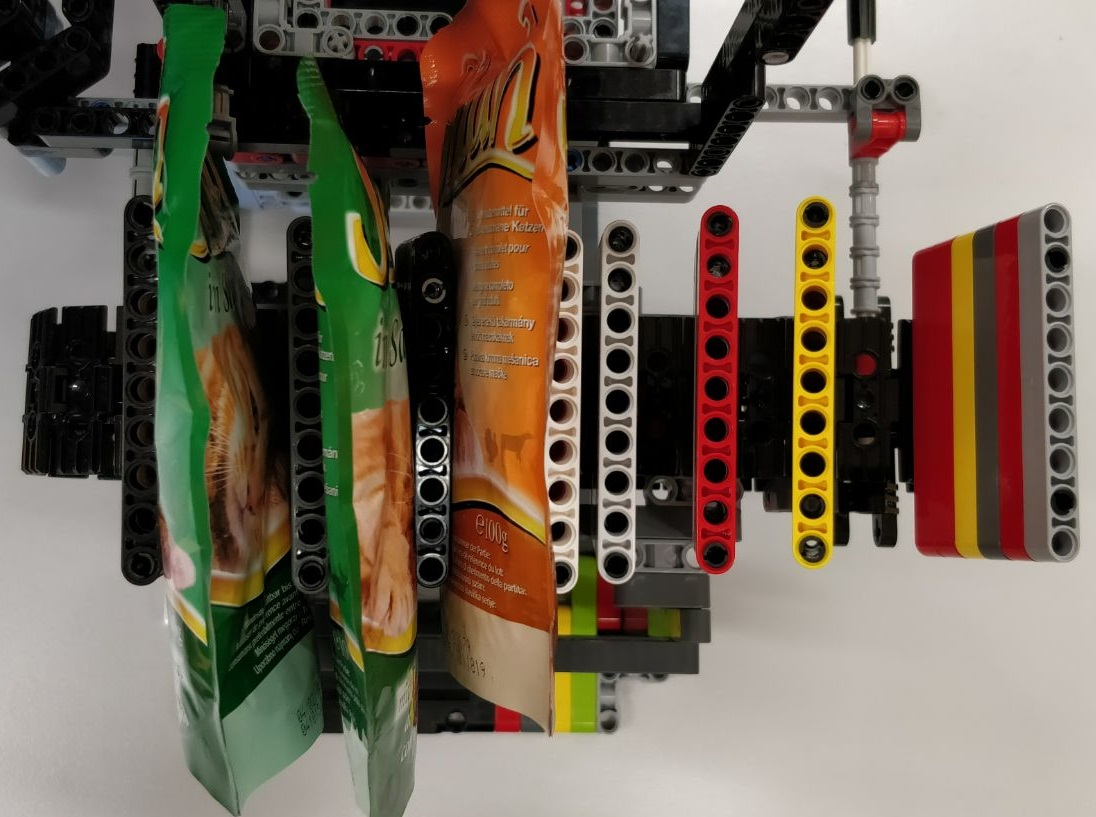
\includegraphics[width=13cm]{Bilder/Ablauf_1_png/Magazin_Oben.jpeg}
\caption{Magazin Oben}
\label{Magazin Oben}
\end{center}
\end{figure}

\newpage 

\subsubsection{Führen zur Schneidplatte}

In diesem Schritt wird mithilfe eines Greifers (dargestellt durch eine Hand) die Packung in richtiger Position gebracht. Siehe Abbildungen: \ref{Magazin Auszug}, \ref{Magazin Mitte}

\begin{figure}[H]
\begin{center}
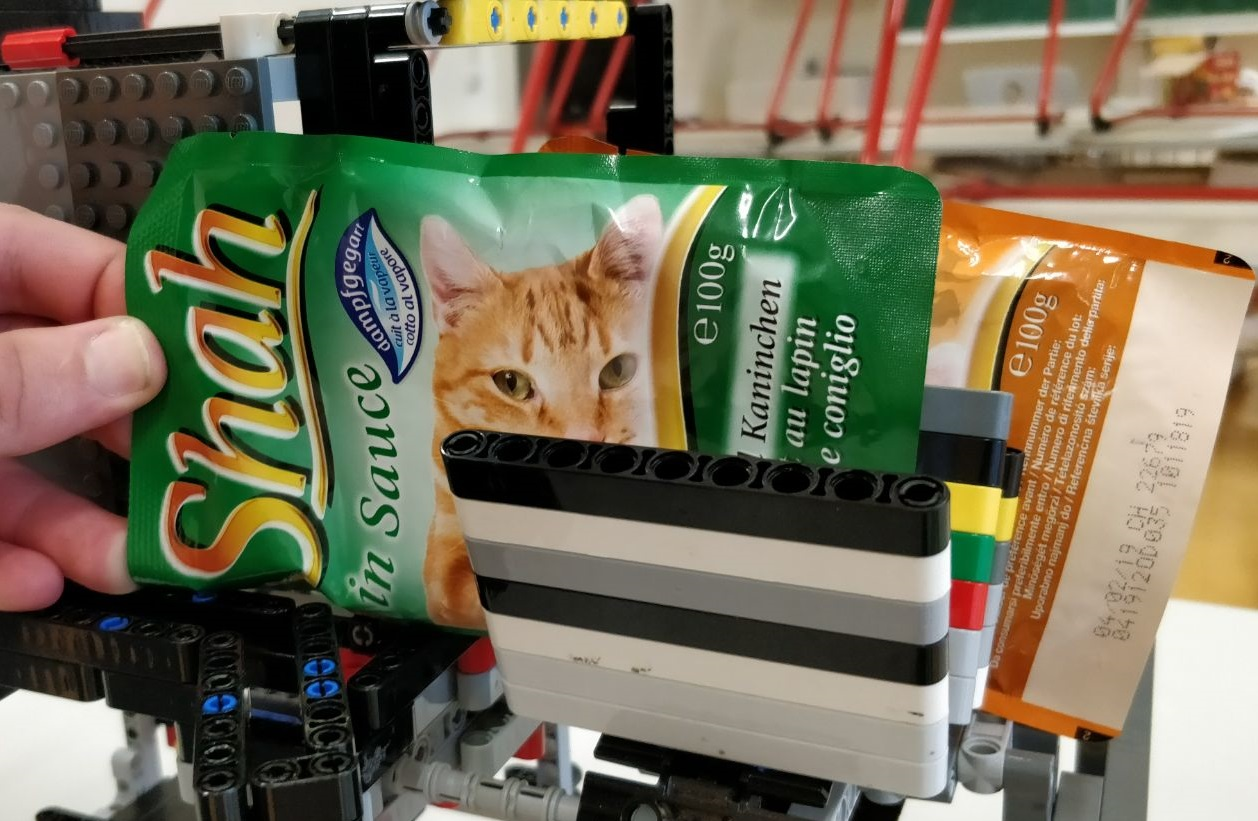
\includegraphics[width=13cm]{Bilder/Ablauf_1_png/Magazin_Auszug.jpeg}
\caption{Magazin Auszug}
\label{Magazin Auszug}
\end{center}
\end{figure}

\begin{figure}[H]
\begin{center}
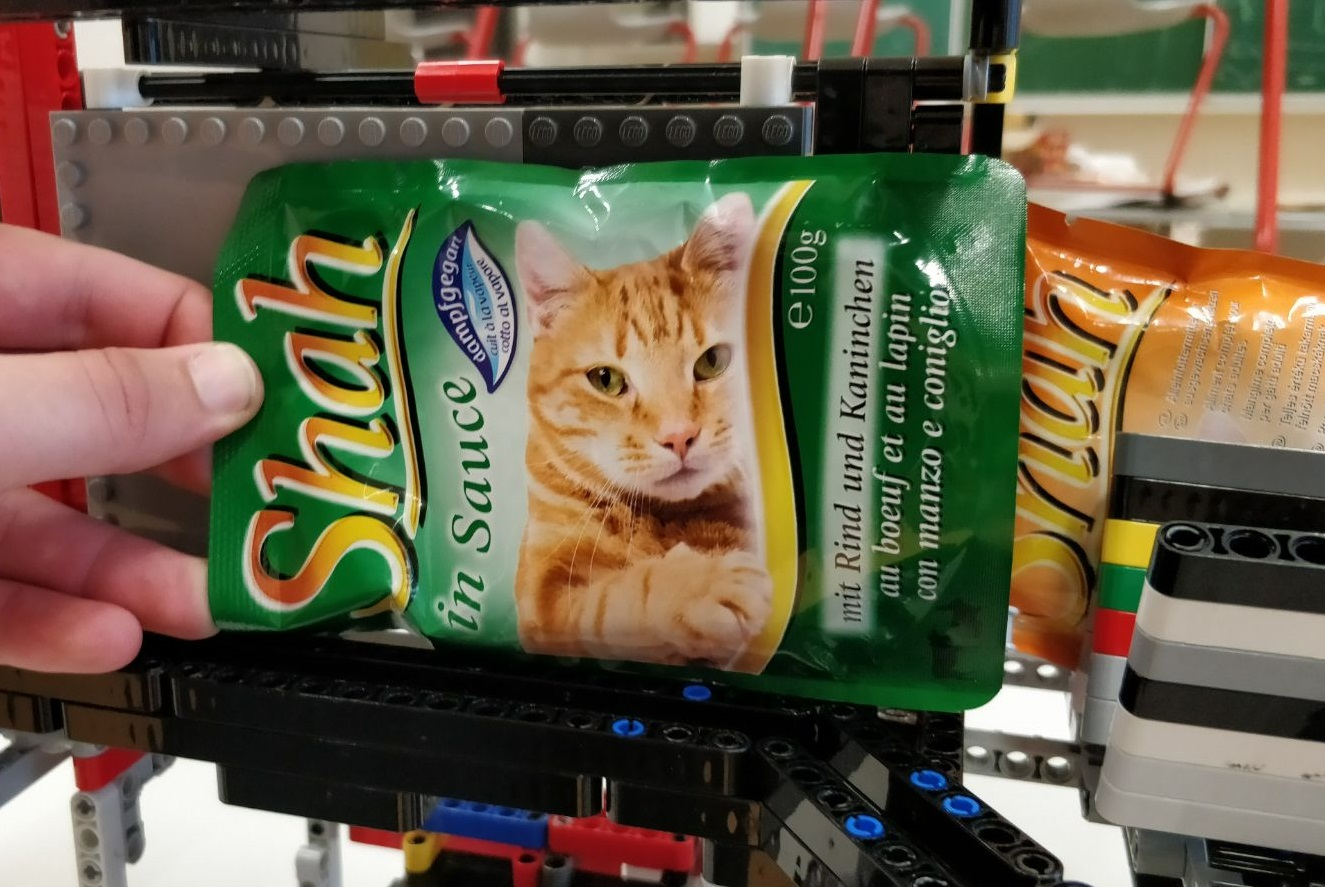
\includegraphics[width=13cm]{Bilder/Ablauf_1_png/Magazin_Auszug_2.jpeg}
\caption{Magazin Auszug Mitte}
\label{Magazin Mitte}
\end{center}
\end{figure}

Wie im Bild gezeigt liegt das Katzenfutterpackerl in der richtigen Position und wird mit zwei Magnetzylindern an der Schneidefläche festgehalten. Siehe Abbildung: \ref{Schneidebereit}

\begin{figure}[H]
\begin{center}
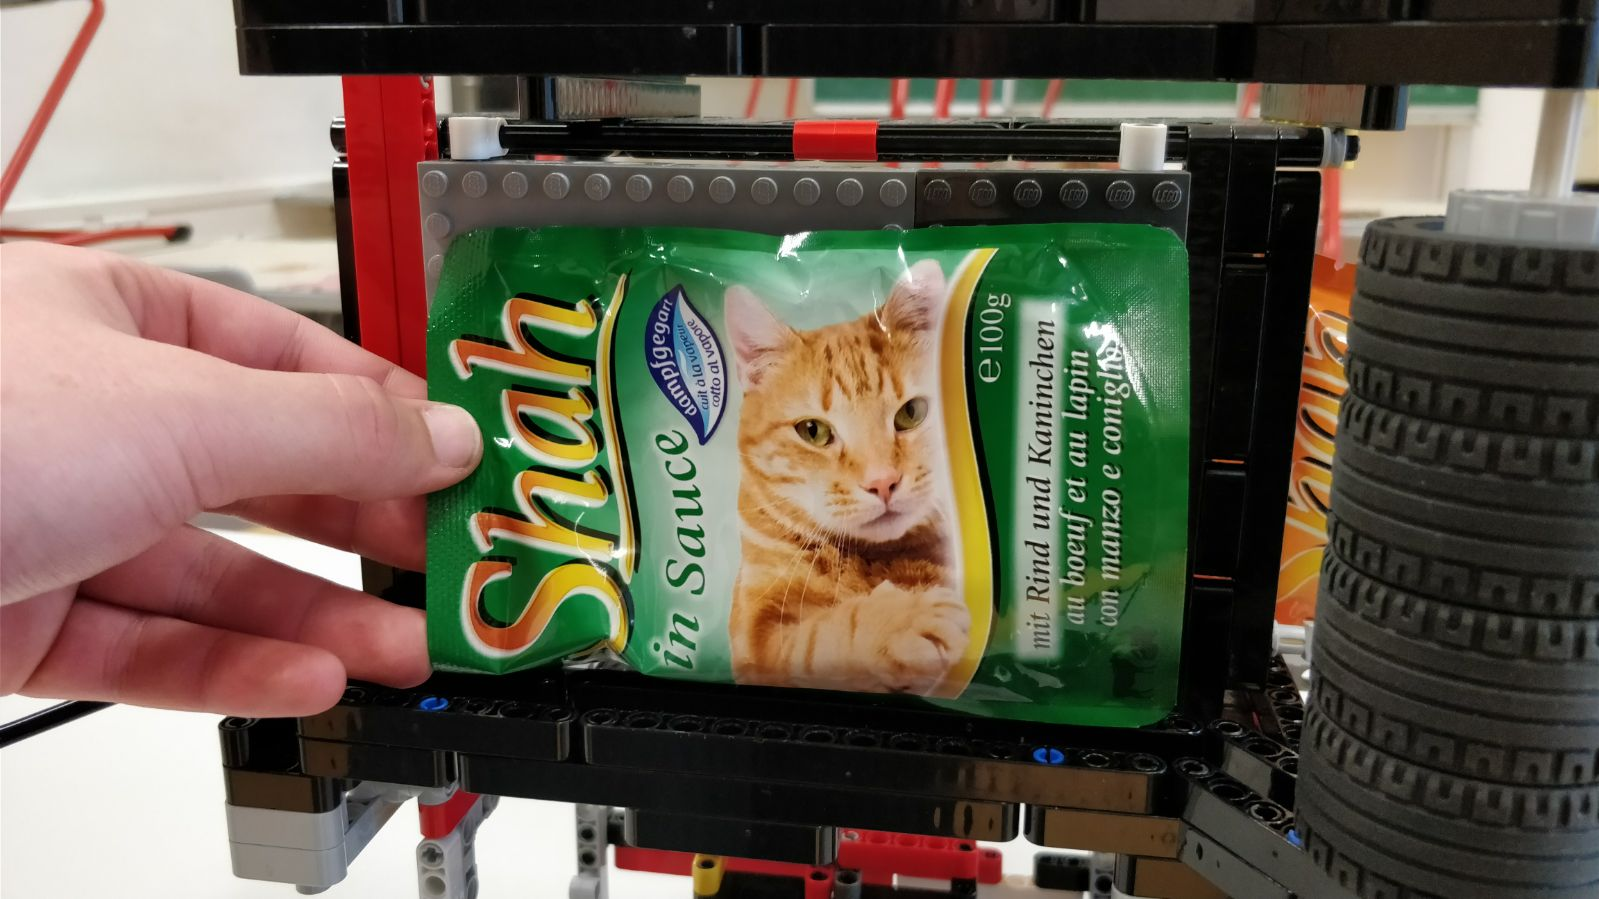
\includegraphics[width=13cm]{Bilder/Ablauf_1_png/Schneidebereit.jpeg}
\caption{Schneidebereit}
\label{Schneidebereit}
\end{center}
\end{figure}

Endposition des Greifers. Kerbe liegt genau an der richtigen Position. 4 Magnetzylinder halten den Futterbeutel and dieser Position, damit der Beutel während des Schneidens nicht verrutscht. Siehe Abbildung: \ref{Fertig Geschnitten}

\begin{figure}[H]
\begin{center}
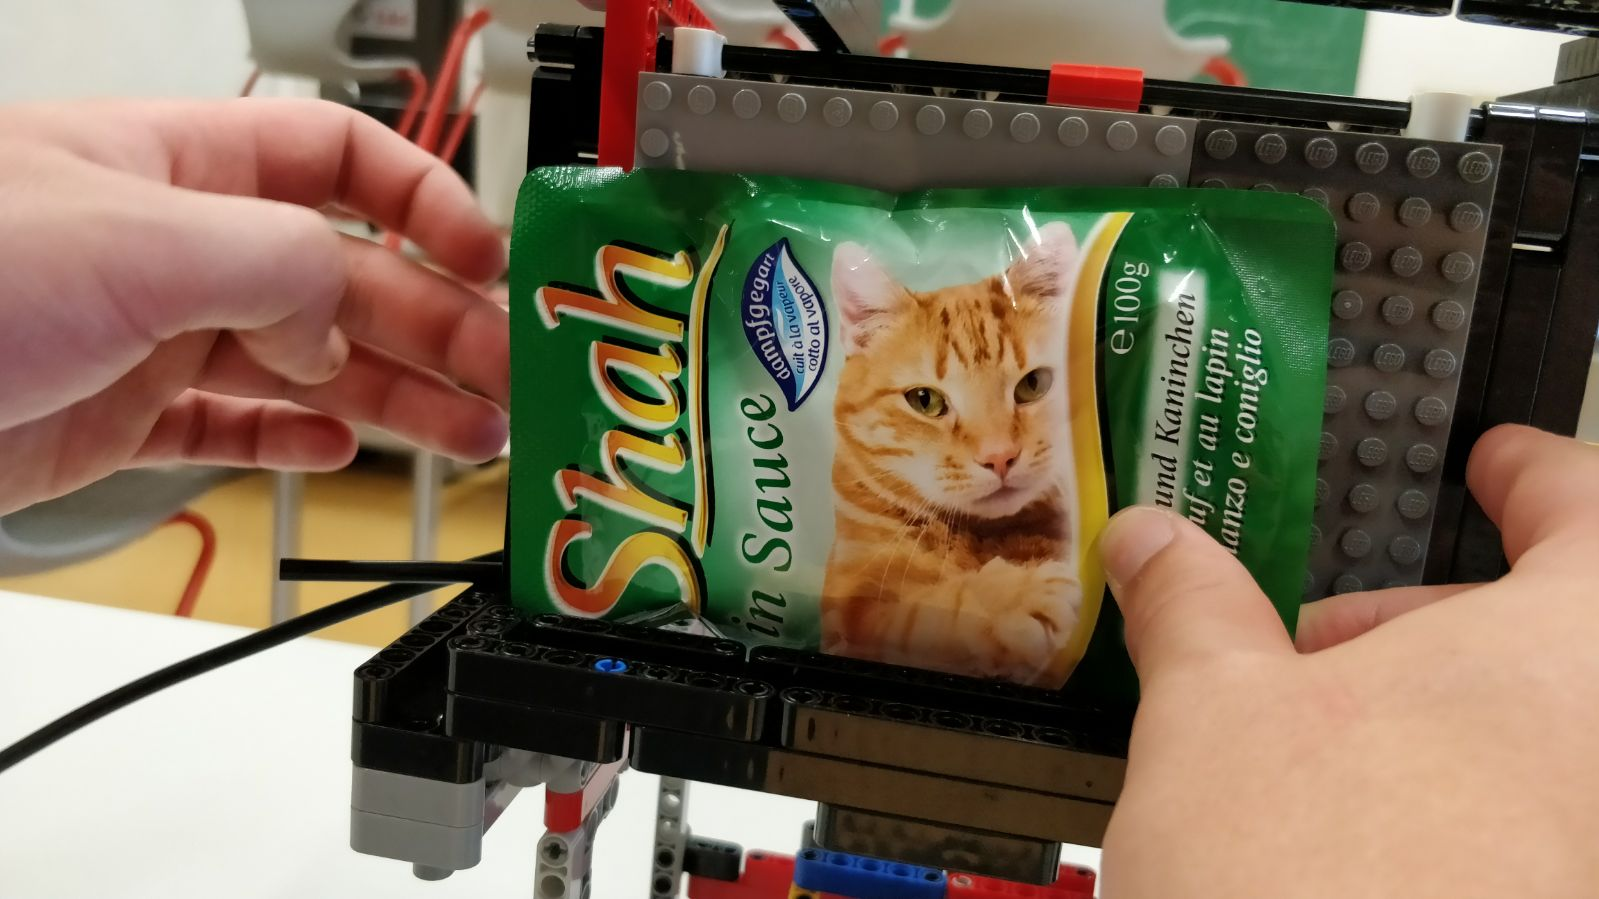
\includegraphics[width=13cm]{Bilder/Ablauf_1_png/Fertig_Geschnitten}
\caption{Fertig Geschnitten}
\label{Fertig Geschnitten}
\end{center}
\end{figure}

\newpage
\subsubsection{Schnitt}

In der richtigen Position muss man mit 2 scharfen Klinge mit viel Druck die Packung aufschneiden. Eine davon wird and der Schnittfläche angebracht und die andere macht die Schneidbewegung, wobei die beiden aneinander reibenden Kanten in einem Schnitt resultieren. Die Packung kann mit einem Schnitt vollständig geöffnet werden. Siehe Abbildung: \ref{Schnitt}

\begin{figure}[H]
\begin{center}
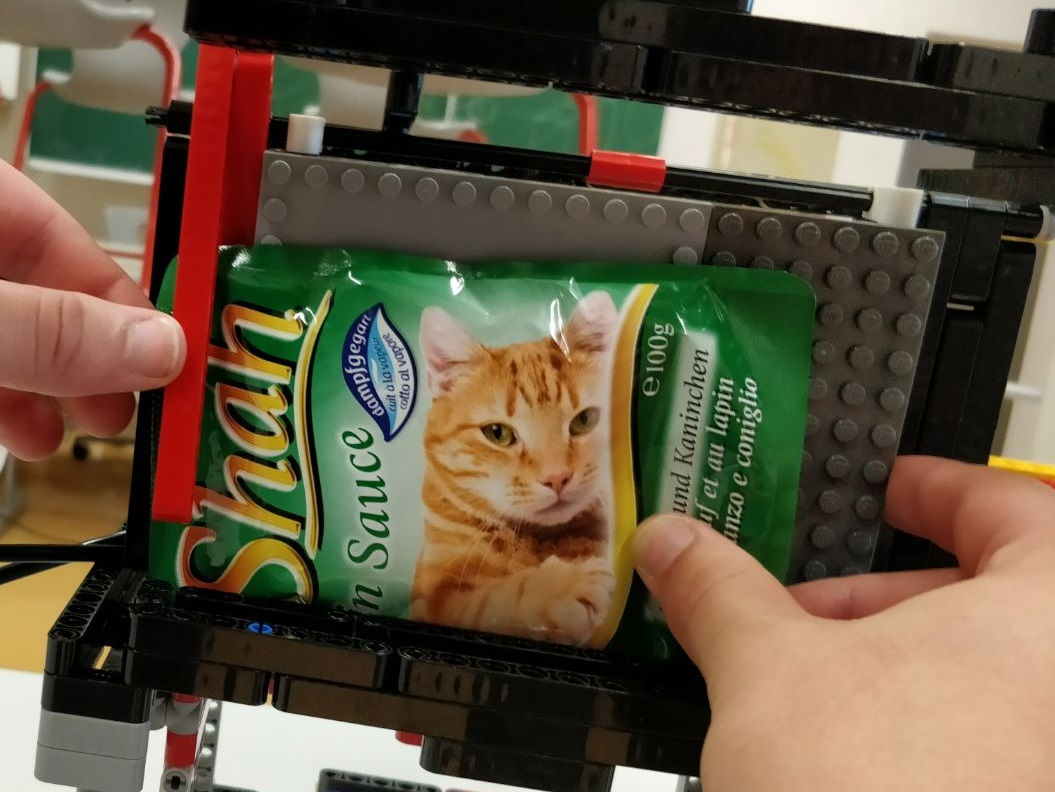
\includegraphics[width=13cm]{Bilder/Ablauf_1_png/Schnitt}
\caption{Schnitt}
\label{Schnitt}
\end{center}
\end{figure} 

\newpage
\subsubsection{Pressen}

Nach dem Aufschneiden wird mit einer Rolle das Sackerl ausgepresst. Dazu werden zuerst die ersten 2 Magnetzylinder gelöst bis die Rolle vorbei ist. Danach werden sie wieder in Position gebracht. Daraufhin werden die anderen beiden gelöst und die Rolle fährt ans Ende. Siehe Abbildungen: \ref{Ausquetschen Beginn}, \ref{Ausquetschen Mitte}, \ref{Ausquetschen Ende}

\begin{figure}[H]
\begin{center}
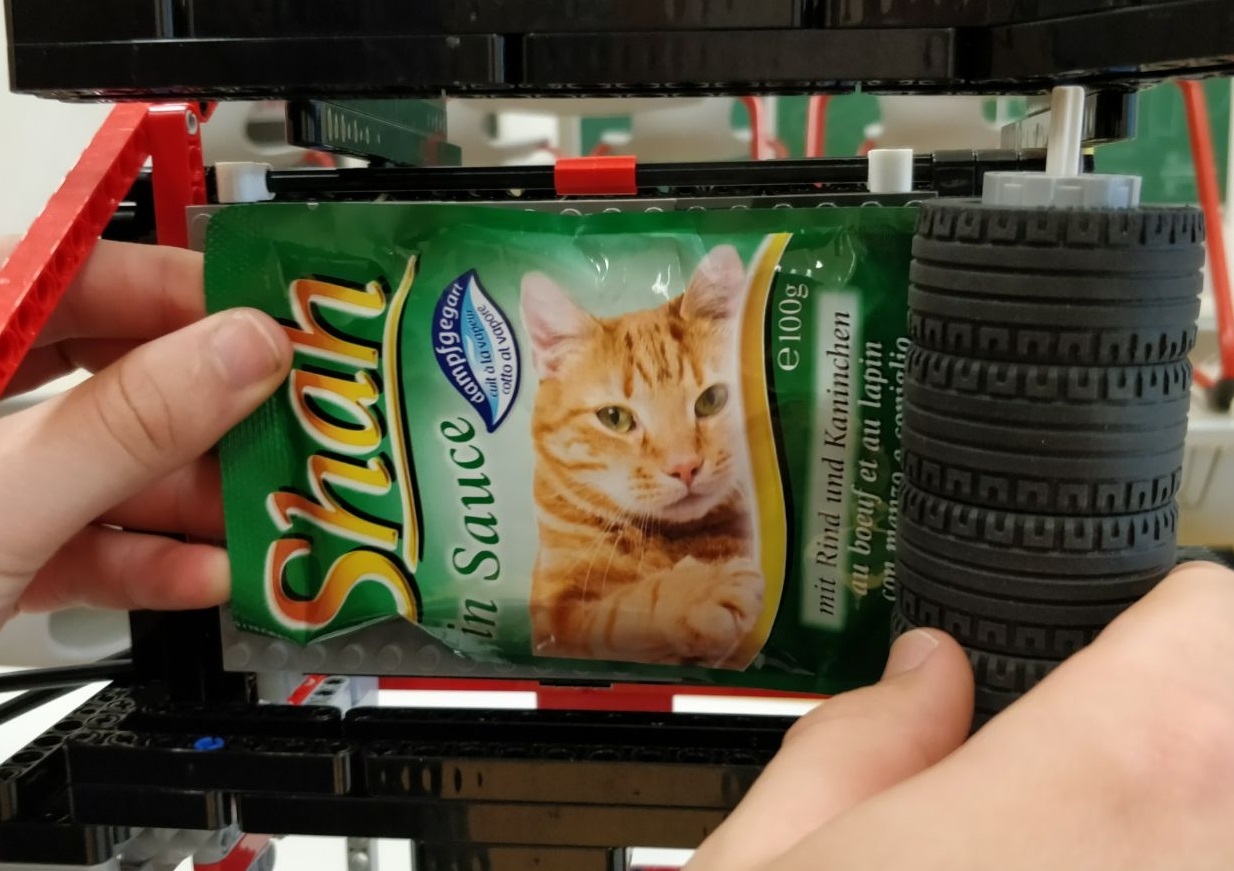
\includegraphics[width=13cm]{Bilder/Ablauf_1_png/Ausquetschen_1}
\caption{Ausquetschen Beginn}
\label{Ausquetschen Beginn}
\end{center}
\end{figure}

\begin{figure}[H]
\begin{center}
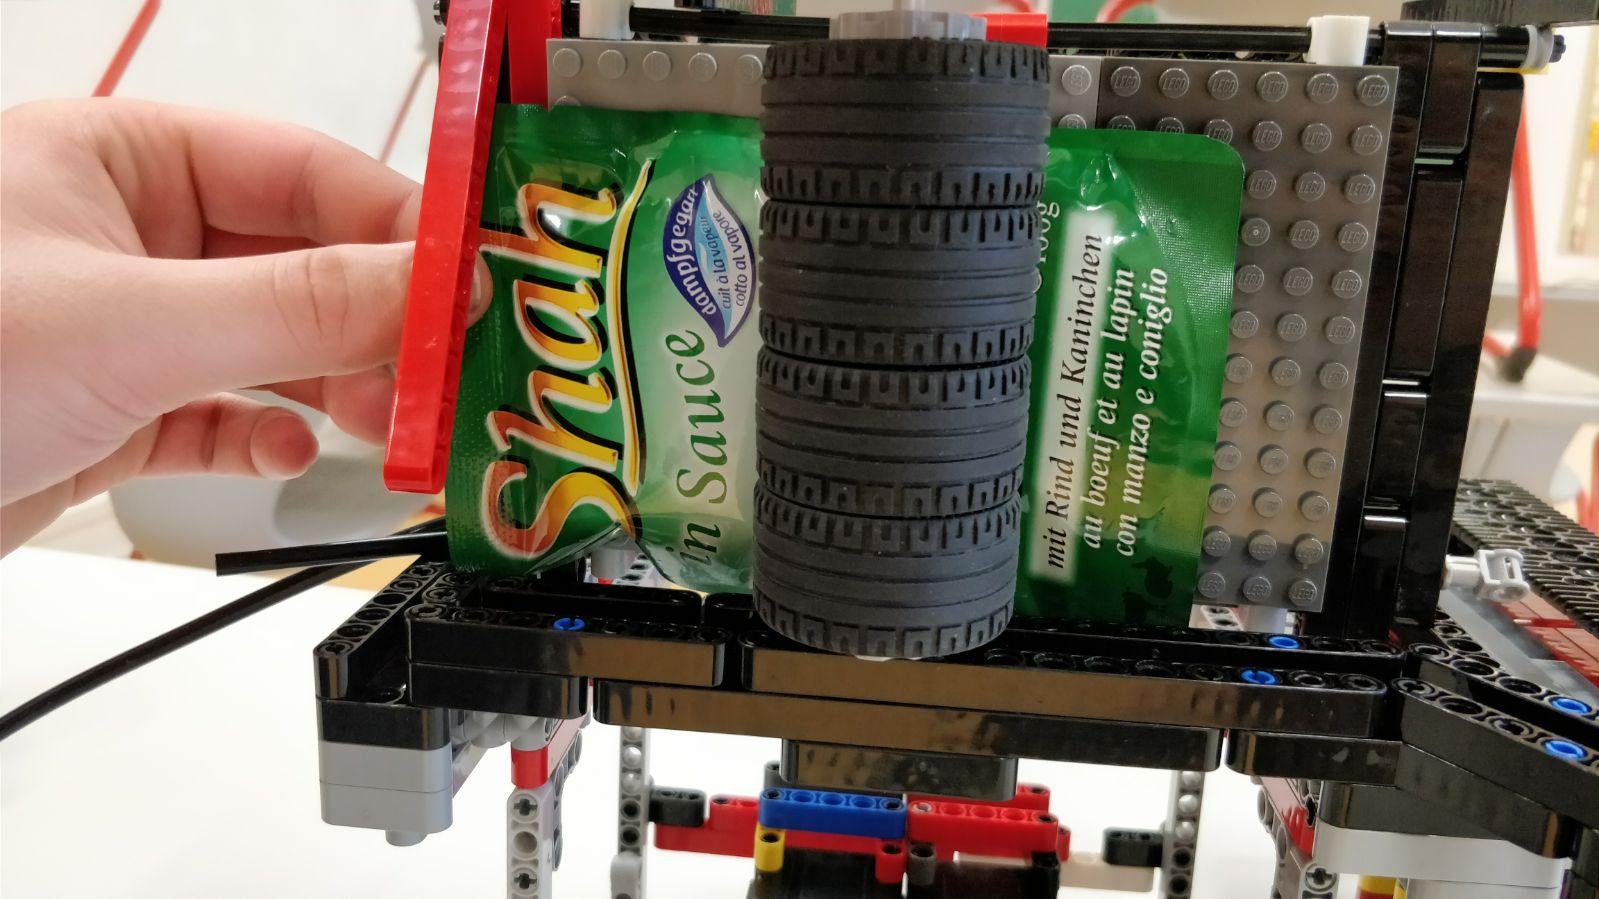
\includegraphics[width=13cm]{Bilder/Ablauf_1_png/Ausquetschen_2}
\caption{Ausquetschen Mitte}
\label{Ausquetschen Mitte}
\end{center}
\end{figure}

\begin{figure}[H]
\begin{center}
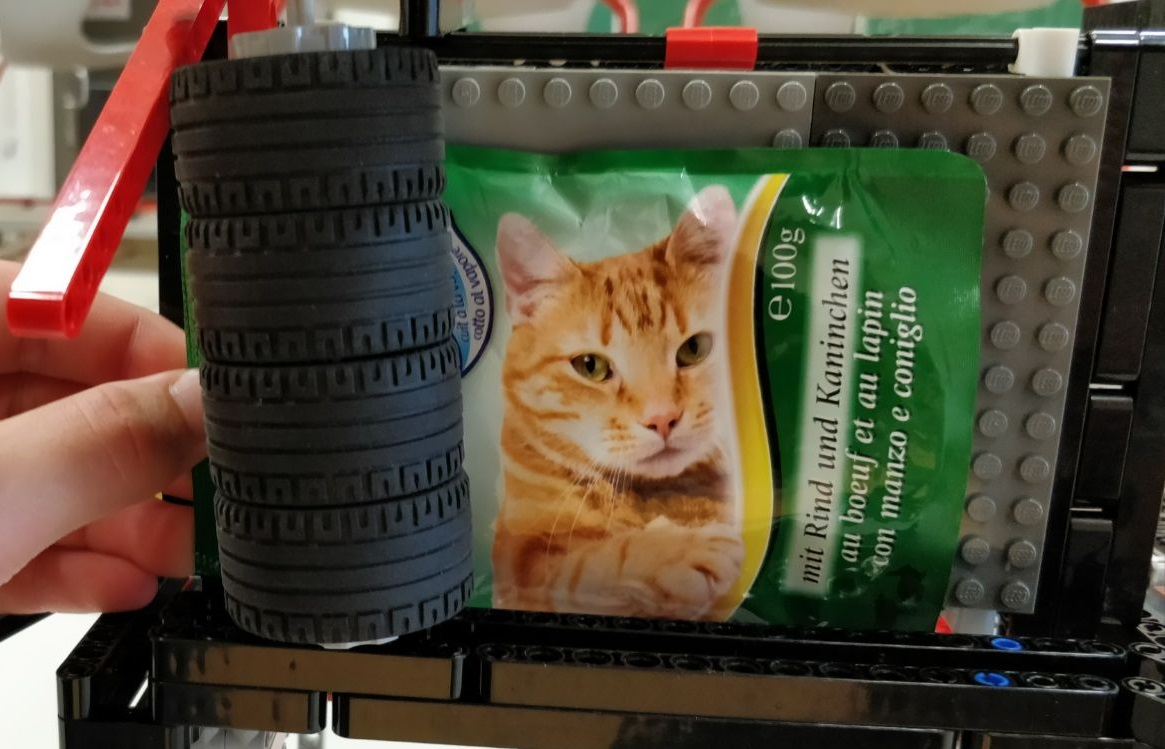
\includegraphics[width=13cm]{Bilder/Ablauf_1_png/Ausquetschen_3}
\caption{Ausquetschen Ende}
\label{Ausquetschen Ende}
\end{center}
\end{figure}
\newpage
\subsubsection{Entsorgen}

Nach dem Auspressen wird die leere Packung durch die Rückklappe in einen Luftdichten Container geworfen. Die Klappe wird durch zwei Stifte gehalten und lässt sich durch ein Scharnier nach hinten klappen. Siehe Abbildung: \ref{Auswurf Beginn}, \ref{Fertiger Auswurf}

\begin{figure}[H]
\begin{center}
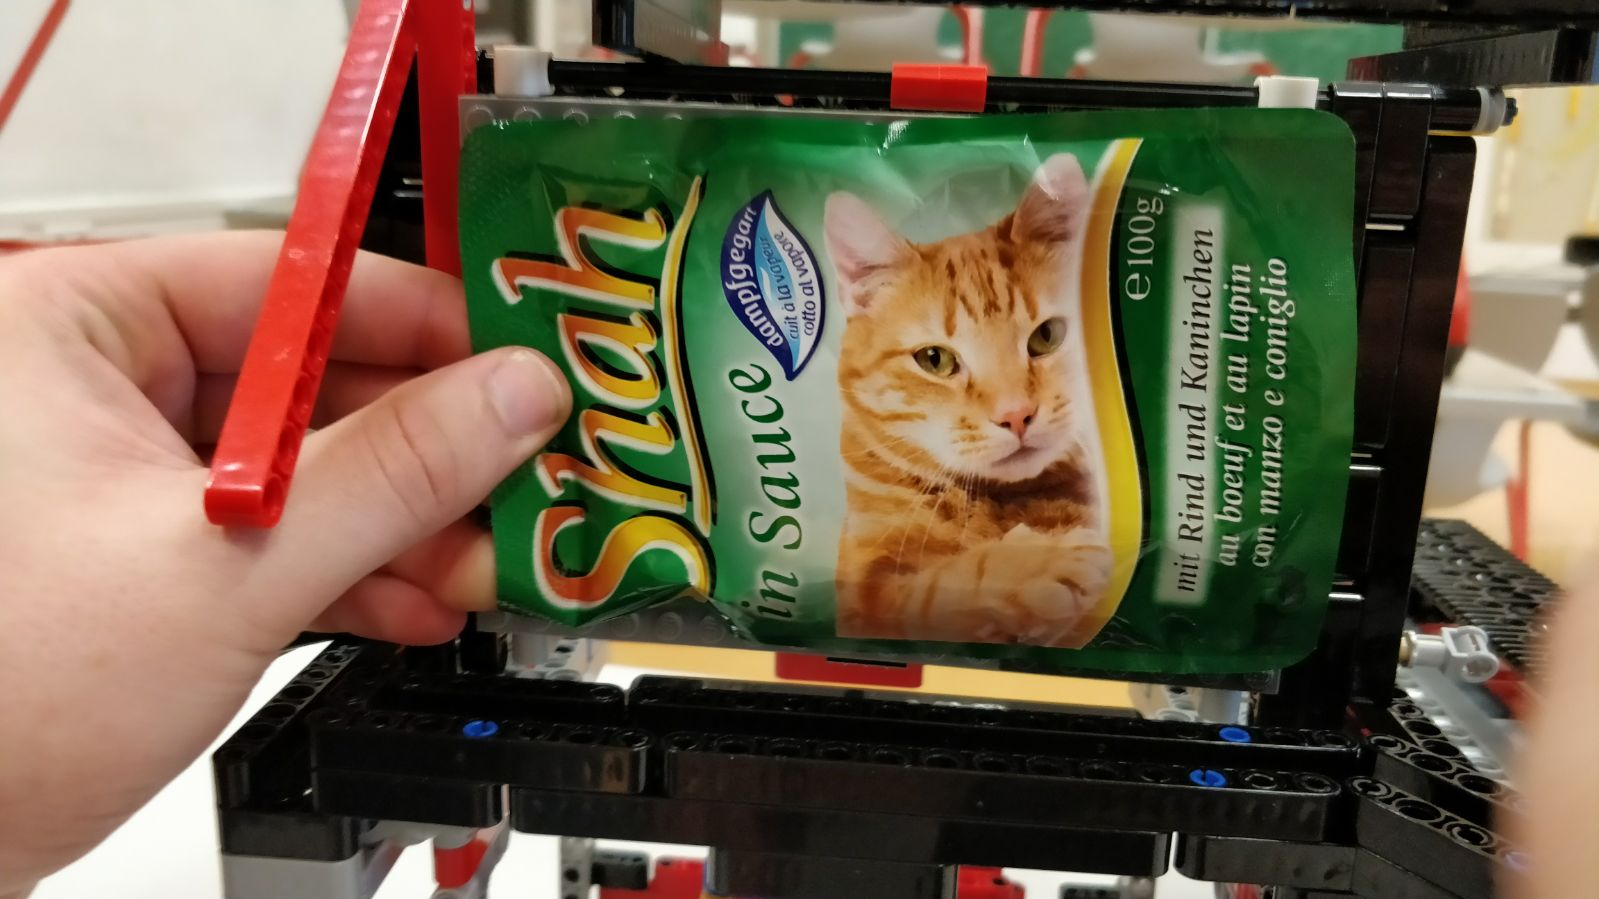
\includegraphics[width=13cm]{Bilder/Ablauf_1_png/Auswurf_1}
\caption{Auswurf Beginn}
\label{Auswurf Beginn}
\end{center}
\end{figure}

In der Abbildung: \ref{Bolzen drinnen} sieht man den Stift der ein vorzeitiges nach Hinten klappen verhindert.

\begin{figure}[H]
\begin{center}
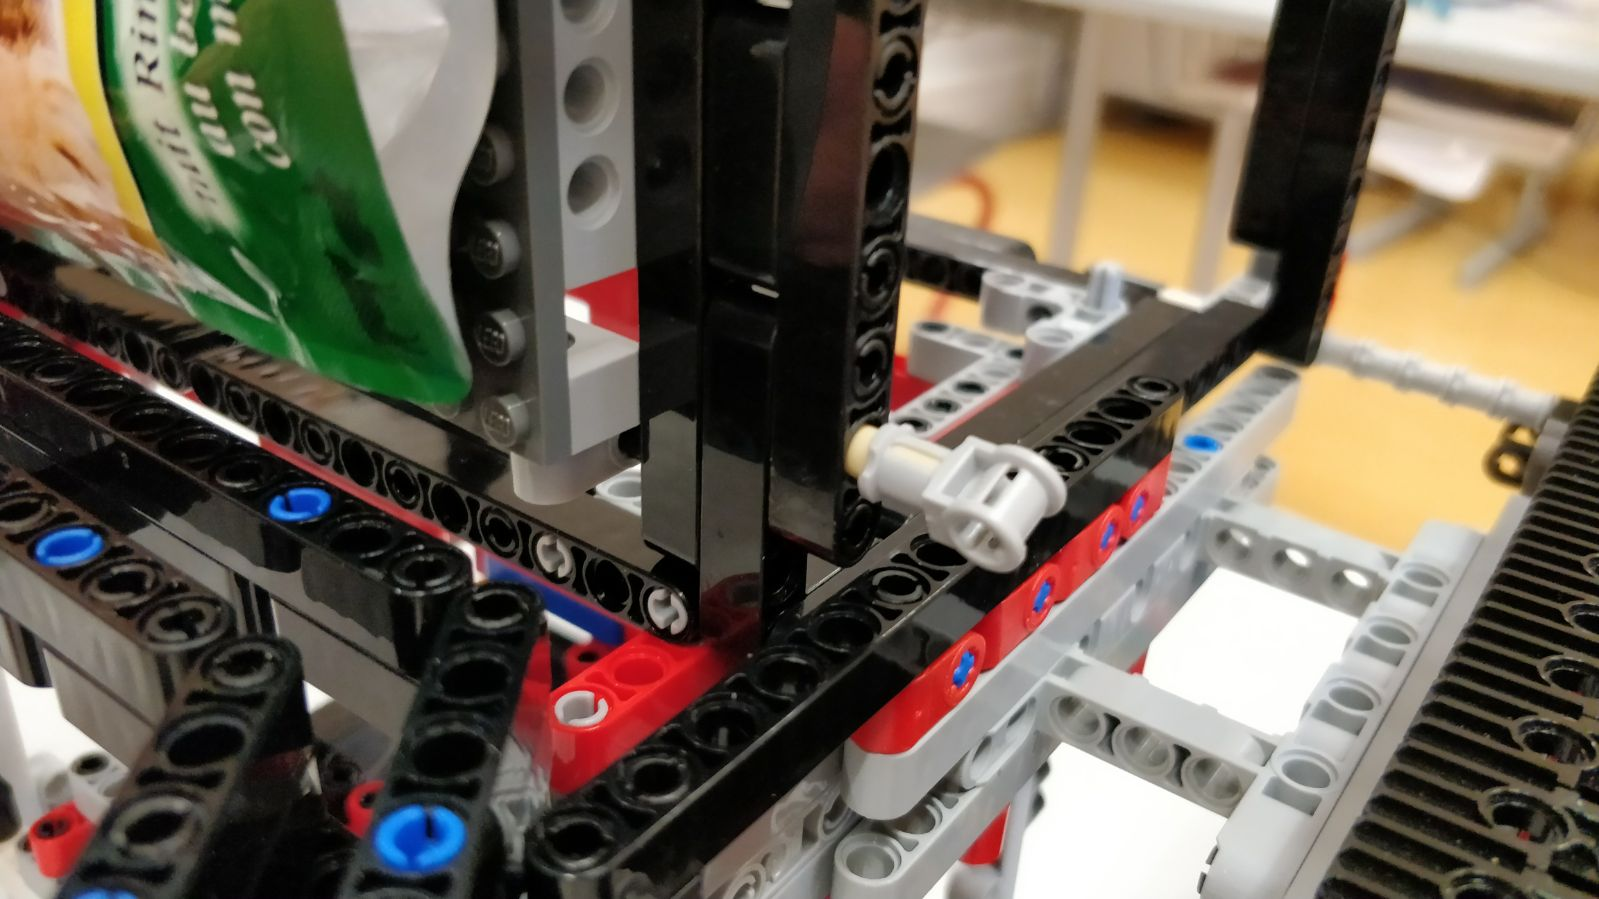
\includegraphics[width=13cm]{Bilder/Ablauf_1_png/Auswurf_2}
\caption{Bolzen drinnen}
\label{Bolzen drinnen}
\end{center}
\end{figure}


In der Abbildung: \ref{Bolzen entfernen} wurde der Bolzen entfernt und somit lässt sich die Klappe nach hinten klappen.

\begin{figure}[H]
\begin{center}
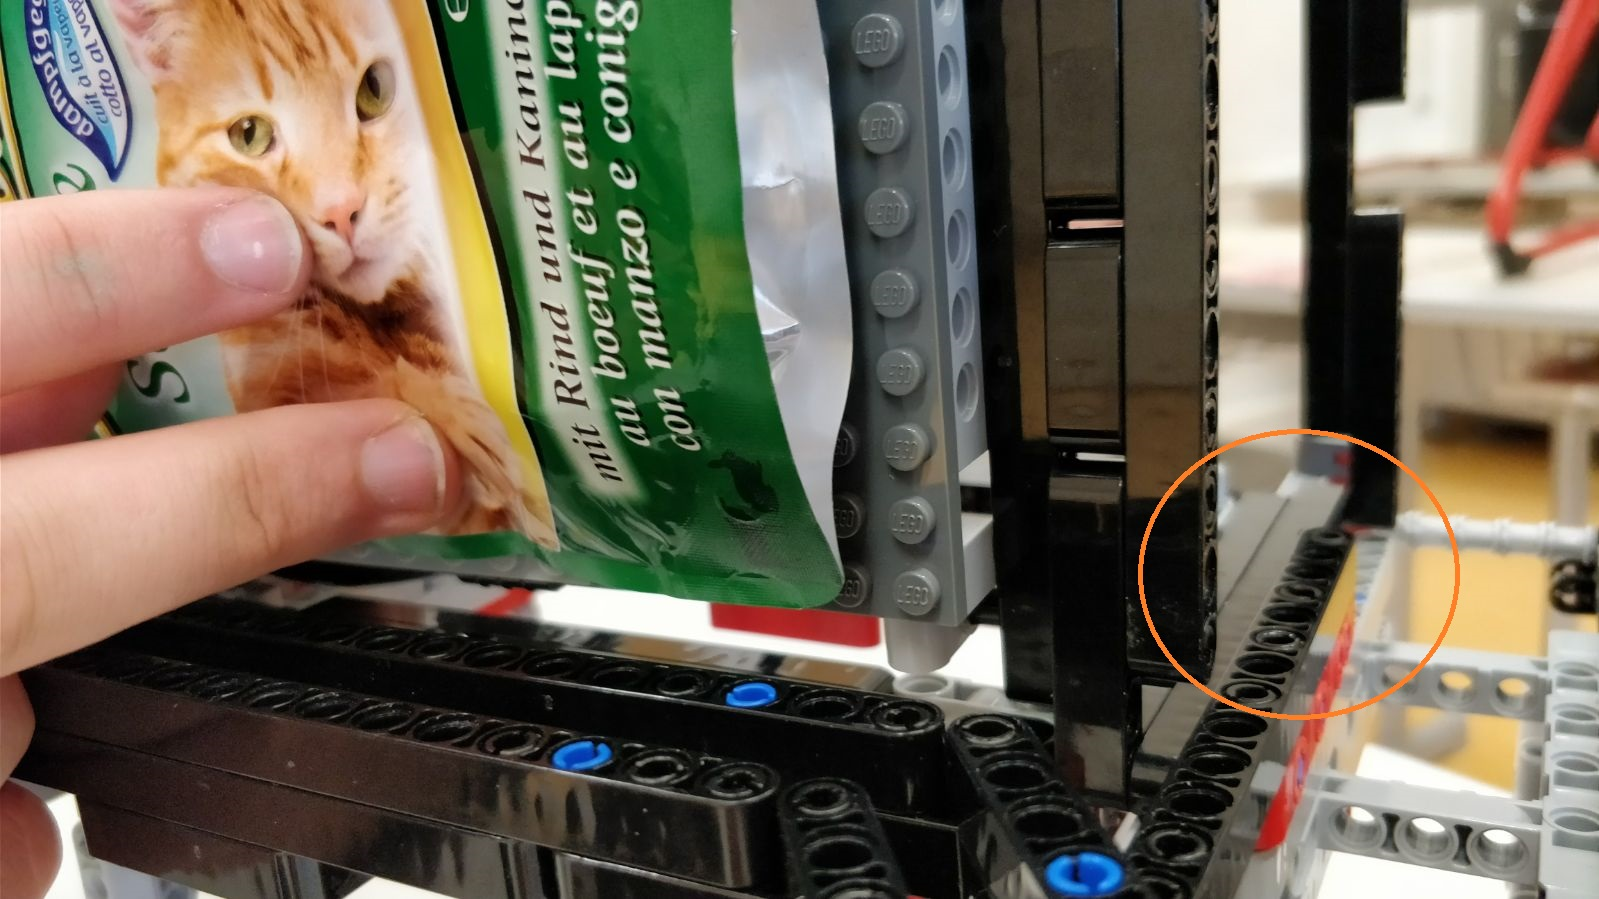
\includegraphics[width=13cm]{Bilder/Ablauf_1_png/Auswurf_3}
\caption{Bolzen entfernen}
\label{Bolzen entfernen}
\end{center}
\end{figure}

In der Abbildung: \ref{Klappe öffnen} wird demonstriert wie die Magnetzylinder die leere Packung gegen die Klappe drücken, wodurch die Klappe sich öffnet.

\begin{figure}[H]
\begin{center}
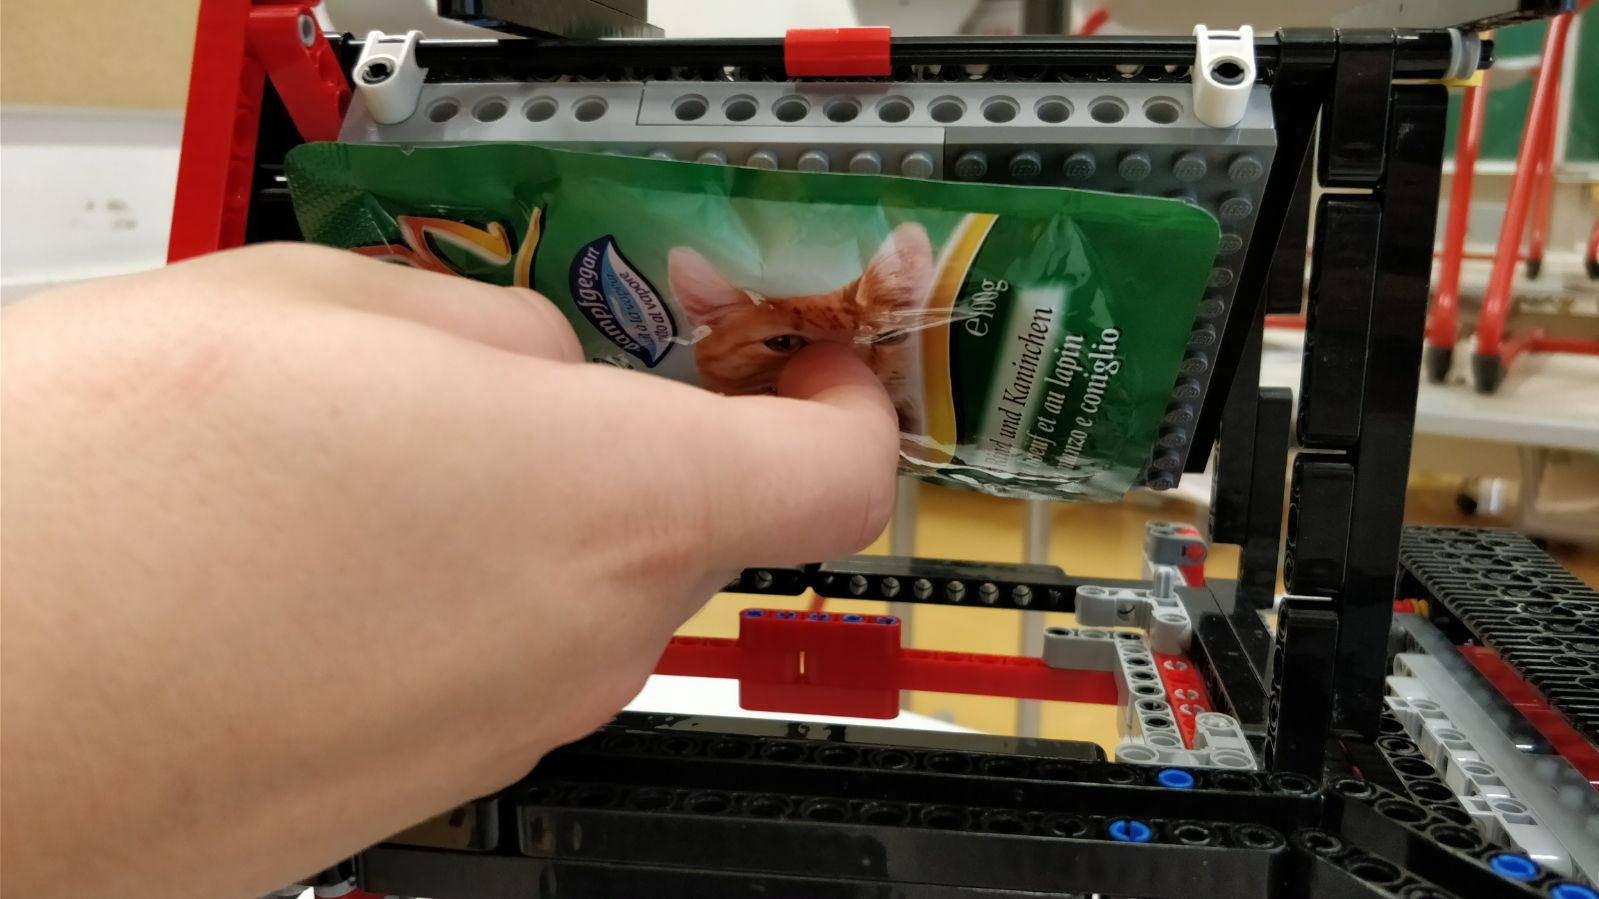
\includegraphics[width=13cm]{Bilder/Ablauf_1_png/Auswurf_4}
\caption{Klappe öffnen}
\label{Klappe öffnen}
\end{center}
\end{figure}

\begin{figure}[H]
\begin{center}
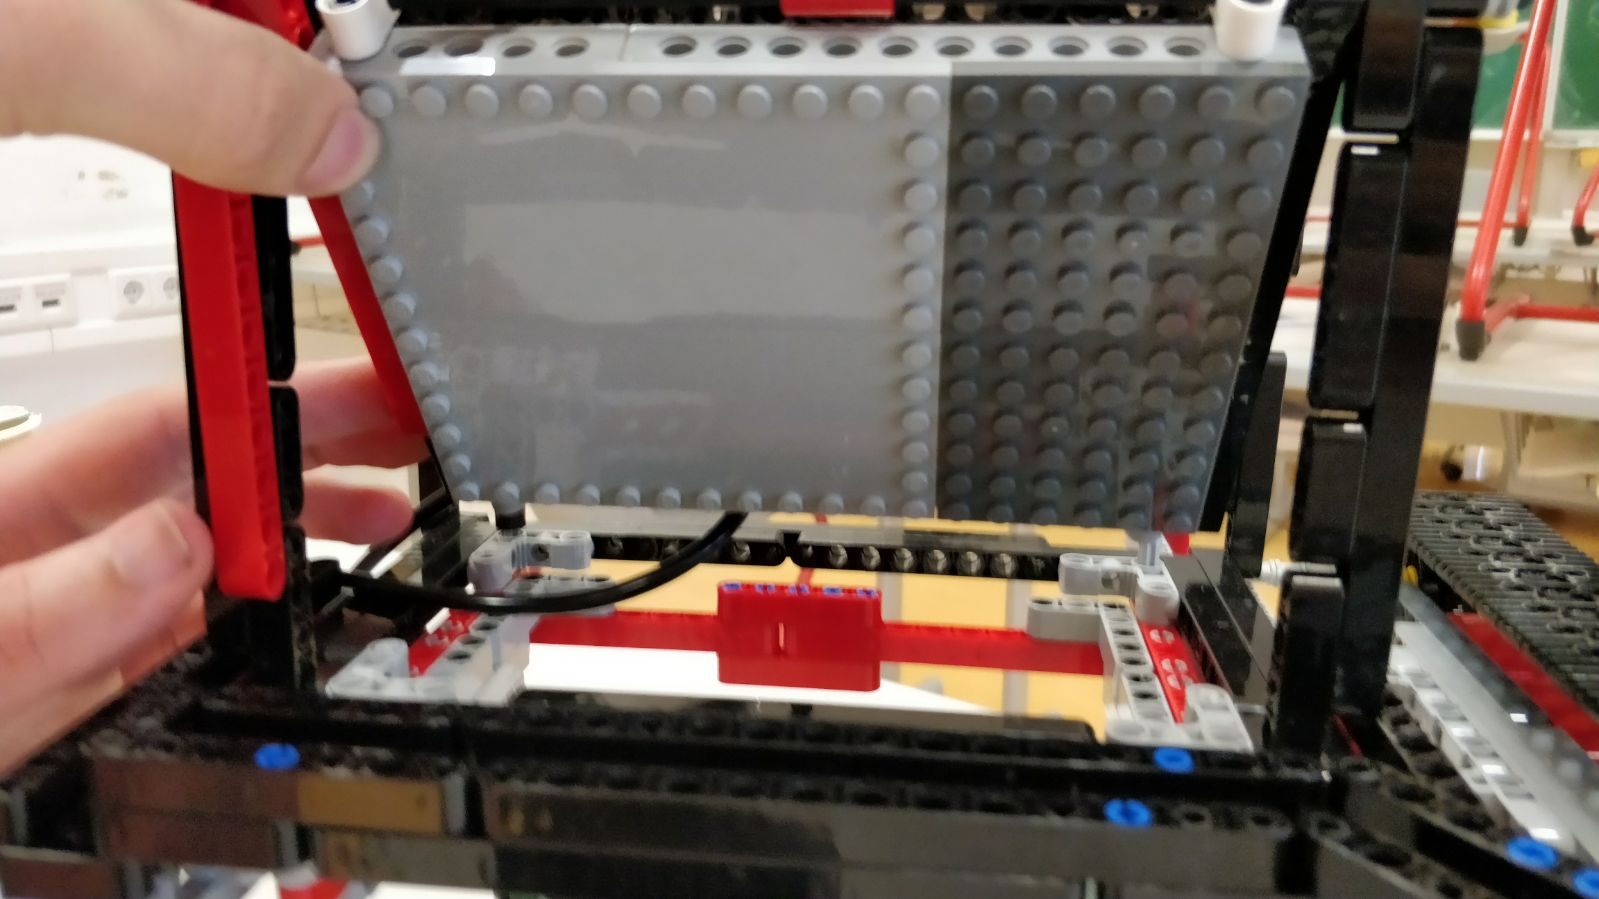
\includegraphics[width=13cm]{Bilder/Ablauf_1_png/Auswurf_5}
\caption{Fertiger Auswurf}
\label{Fertiger Auswurf}
\end{center}
\end{figure}

\subsubsection{Füttern}

Die Maschine besitzt 5 Futterschüsseln die auf einer drehbaren Platte stehen. Vor dem Füttern wird eine Saubere Platte unter der Stelle, wo später die Packung aufgeschnitten wird, positioniert. Während des Auspressens wird fliegt das Futter in die Futterschüssel. Wenn der Auspressvorgang beendet ist, wird die Futterschüssel an eine Position bewegt, wo die Katze Zugang zum fressen hat.
\newpage

\subsection{Variante 2}

\subsubsection{Förderband und Kettenglieder}

Beim Förderband erkennt man wo sich die Futterpackungen befinden sollen. Es wird über die zwei Kettenräder eine Kette gespannt. Auf diese Kette werden die Futterpackungen gehängt, dass funktioniert aber nur weil die Kettenglieder einen Rechtenwinkel auf jeder Seite hat (siehe Abbildung: \ref{Kettenglied}. Auf diesen Winkel wird eine Aluplatte geschraubt und mit einer anderen Platte festgeklemmt. Die Kette wird mithilfe eines Motors in Bewegung gebracht, damit bewegt sich die Packung immer näher Richtung Walze. Siehe Abbildung: \ref{Foerderband}

\begin{figure}[H]
   \begin{minipage}[hbt]{.3\linewidth} % [b] => Ausrichtung an \caption
      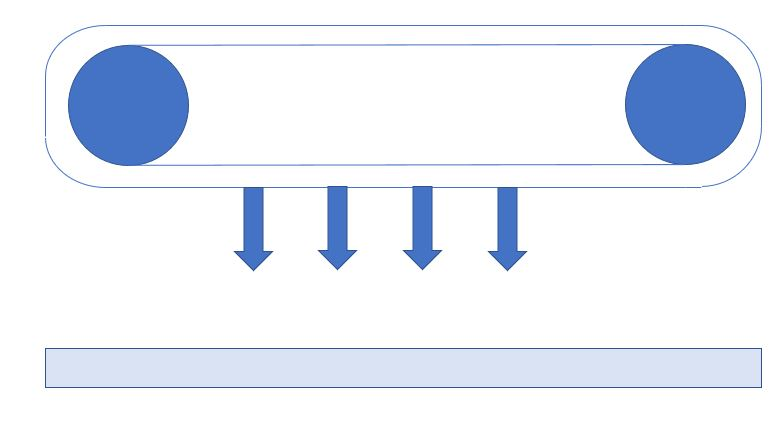
\includegraphics[width=\linewidth]{Bilder/Powerpoint/Foerderband}
      \caption{Foerderband}
      \label{Foerderband}
   \end{minipage}
   \hspace{.3\linewidth}% Abstand zwischen Bilder
   \begin{minipage}[hbt]{.2\linewidth} % [b] => Ausrichtung an \caption
      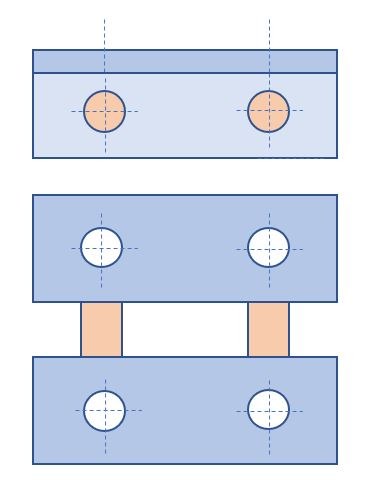
\includegraphics[width=\linewidth]{Bilder/Powerpoint/Kettenglied}
      \caption{Kettenglied}
	  \label{Kettenglied}      
      \end{minipage}
\end{figure}

\subsection{Variante 3}

In dieser Variante wurde überlegt, ob man das Futter nicht einfrieren kann, dieses danach aus der Gefriertruhe holt und erwärmt. Der Vorteil hierbei ist es können keine Schädlinge in das Futter gelange da es tiefgefroren ist und es kann die Portionsgröße eingestellt werden wieviel die Katze bekommt da der Benutzer die Menge an Futter selbst bestimmen kann.  Weiters müsste man nicht über das Schneide Problem nachdenken, da es eine knifflige Anglegenheit ist die Packung bei jeden Schnitt perfekt zu schneiden. Der große Nachteil ist der Platzbedarf und der hohe Energieverbrauch der Kühltruhe. Auch die Entnahme des Futters aus der Kühltruhe ist kein leichtes Unterfangen, da man entwerder viel mit Magnetzylinder arbeiten muss zur Verschiebung der Abdeckung oder ein Loch aus dem der Greifer das Futter entnimmt und dicht Halten muss, damit die Kühltruhe nicht zu warm wird, alles zerschmiltz und schlussendlich das Futter verdirbt. 

\newpage
\section{Aufbauten und Tests}

In diesem Abschnitt der Diplomarbeit werden verschiedene Tests der obigen Varianten zu sehen sein. \\

\subsection{Fütterungsexperiment} 

In diesem Experiment wurde getestet wie lange es Dauert bis eine Packung nur mit Hilfe der Schwerkraft ausläuft. Der Beutel wurde nicht extra erwärmt und wird nur an den beiden unteren Ecken gehalten. Siehe Abbildungen: \ref{Halterung}, \ref{Fütterungs Anfang}, \ref{Fütterungs Mitte}

\begin{figure}[H]
   \begin{minipage}[hbt]{.4\linewidth} % [b] => Ausrichtung an \caption
      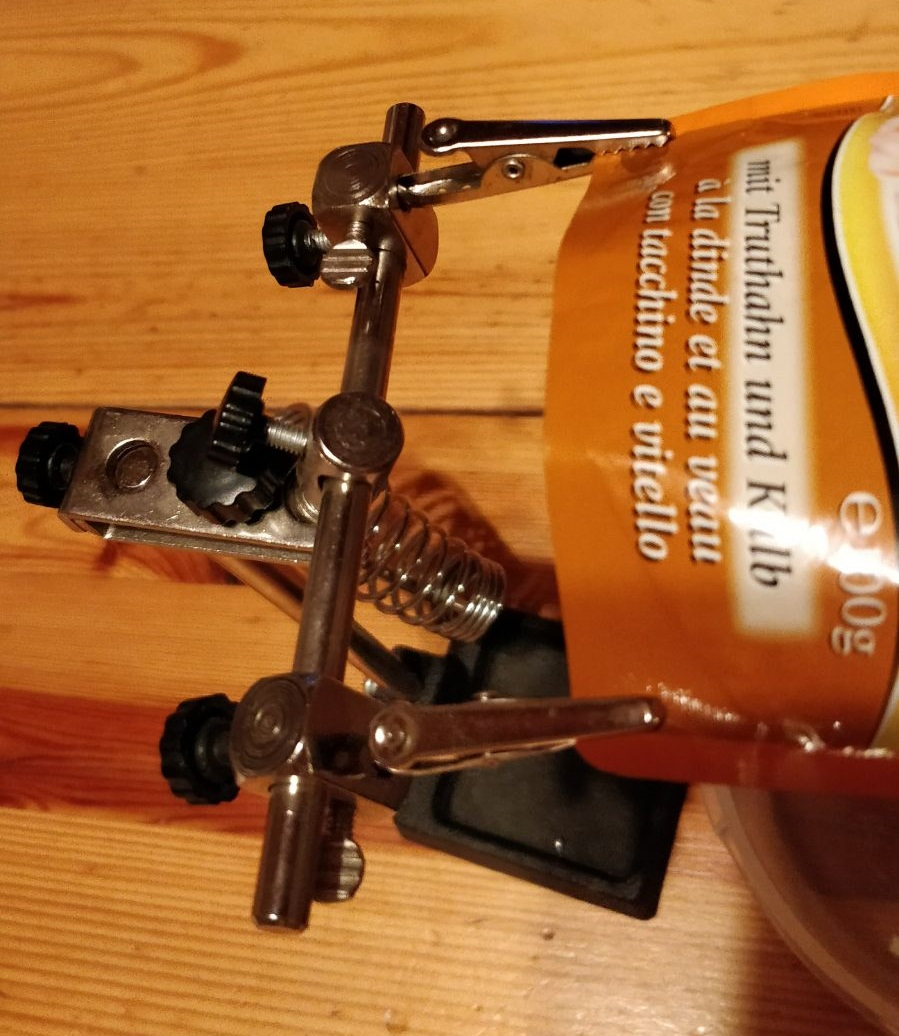
\includegraphics[width=\linewidth]{Bilder/Fuetterungsexperiment/Aufhaengung}
      \caption{Halterung}
      \label{Halterung}
   \end{minipage}
   \hspace{.2\linewidth}% Abstand zwischen Bilder
   \begin{minipage}[hbt]{.4\linewidth} % [b] => Ausrichtung an \caption
      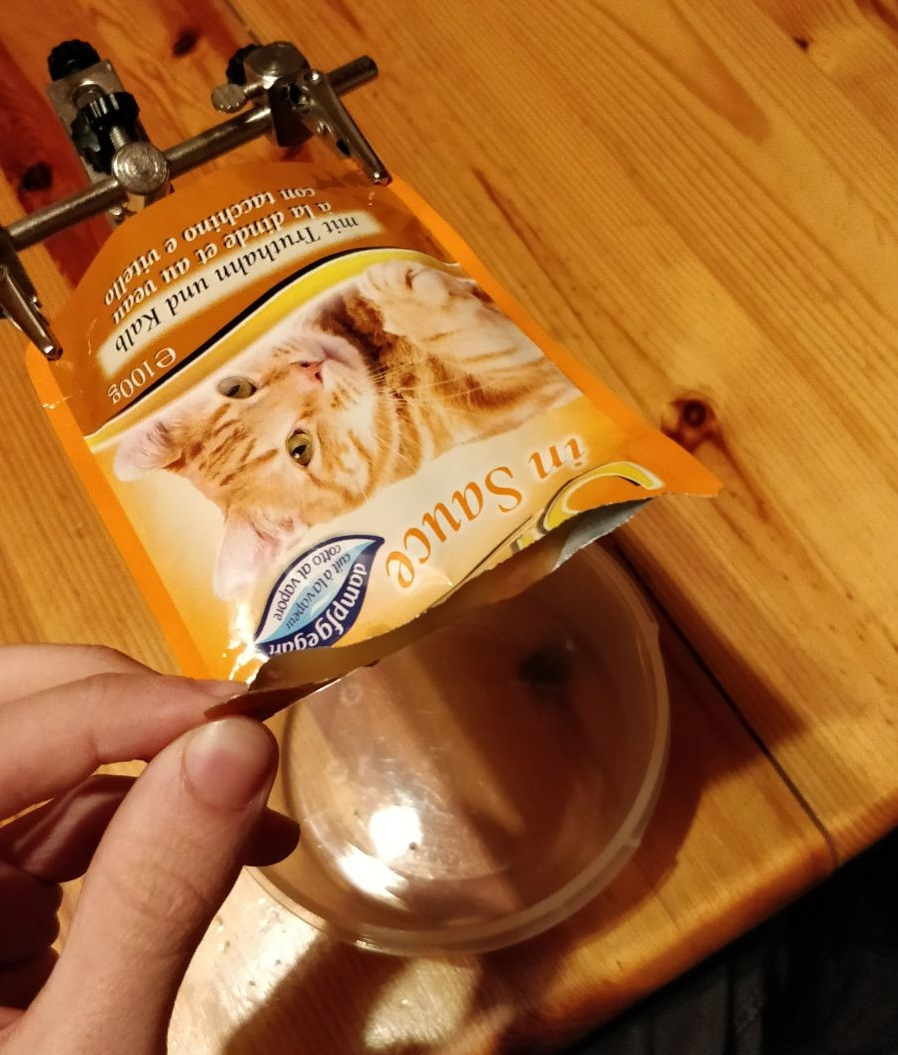
\includegraphics[width=\linewidth]{Bilder/Fuetterungsexperiment/Fuetterungs_Anfang}
      \caption{Fütterungs Anfang}
	  \label{Fütterungs Anfang}      
      \end{minipage}
\end{figure}


\begin{figure}[H]
   \begin{minipage}[hbt]{.3\linewidth} % [b] => Ausrichtung an \caption
      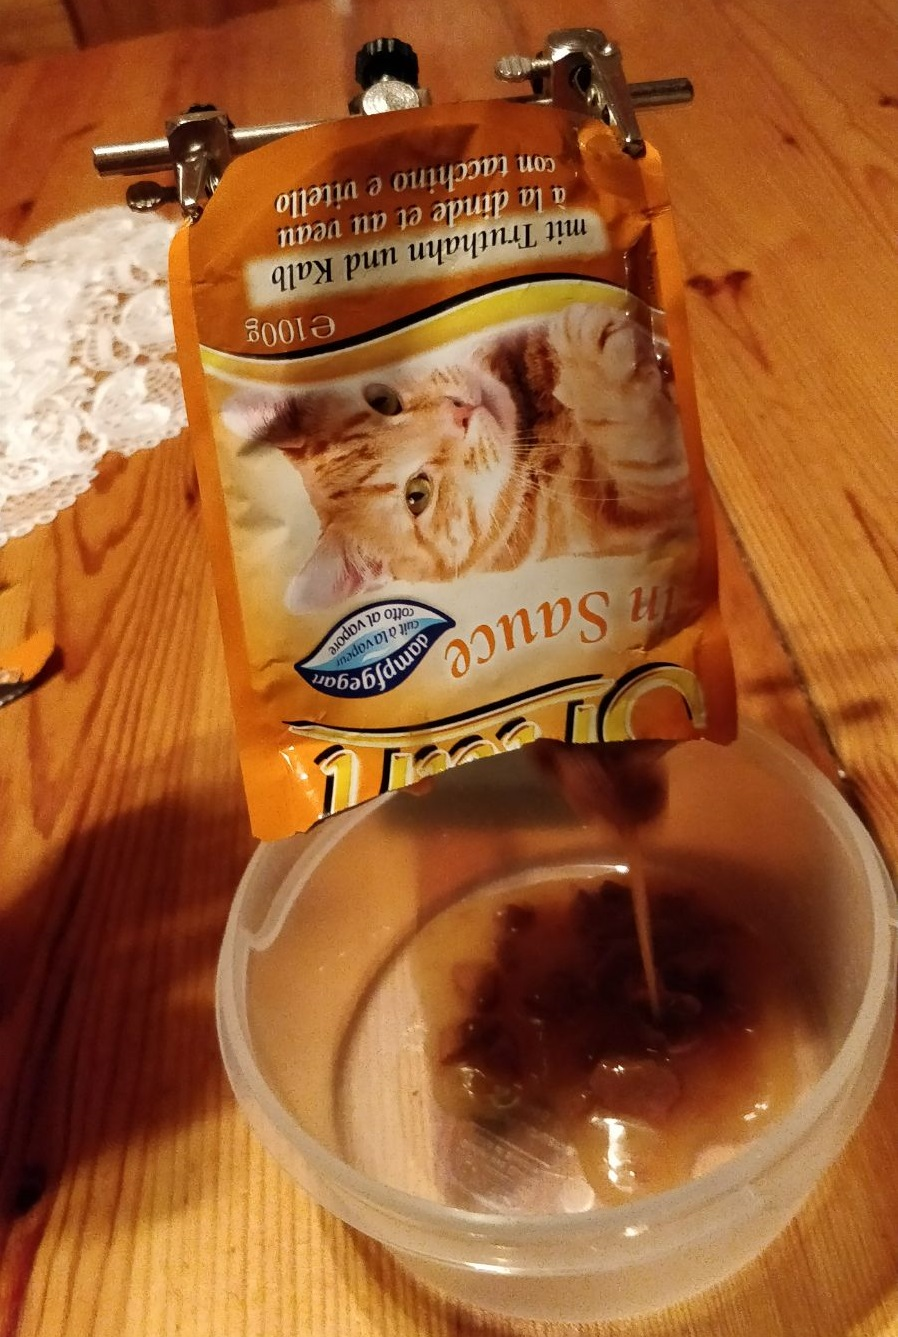
\includegraphics[width=\linewidth]{Bilder/Fuetterungsexperiment/Fuetterungs_Mitte}
      \caption{Fütterungs Mitte}
      \label{Fütterungs Mitte}
   \end{minipage}
   \hspace{.4\linewidth}% Abstand zwischen Bilder
   \begin{minipage}[hbt]{.3\linewidth} % [b] => Ausrichtung an \caption
     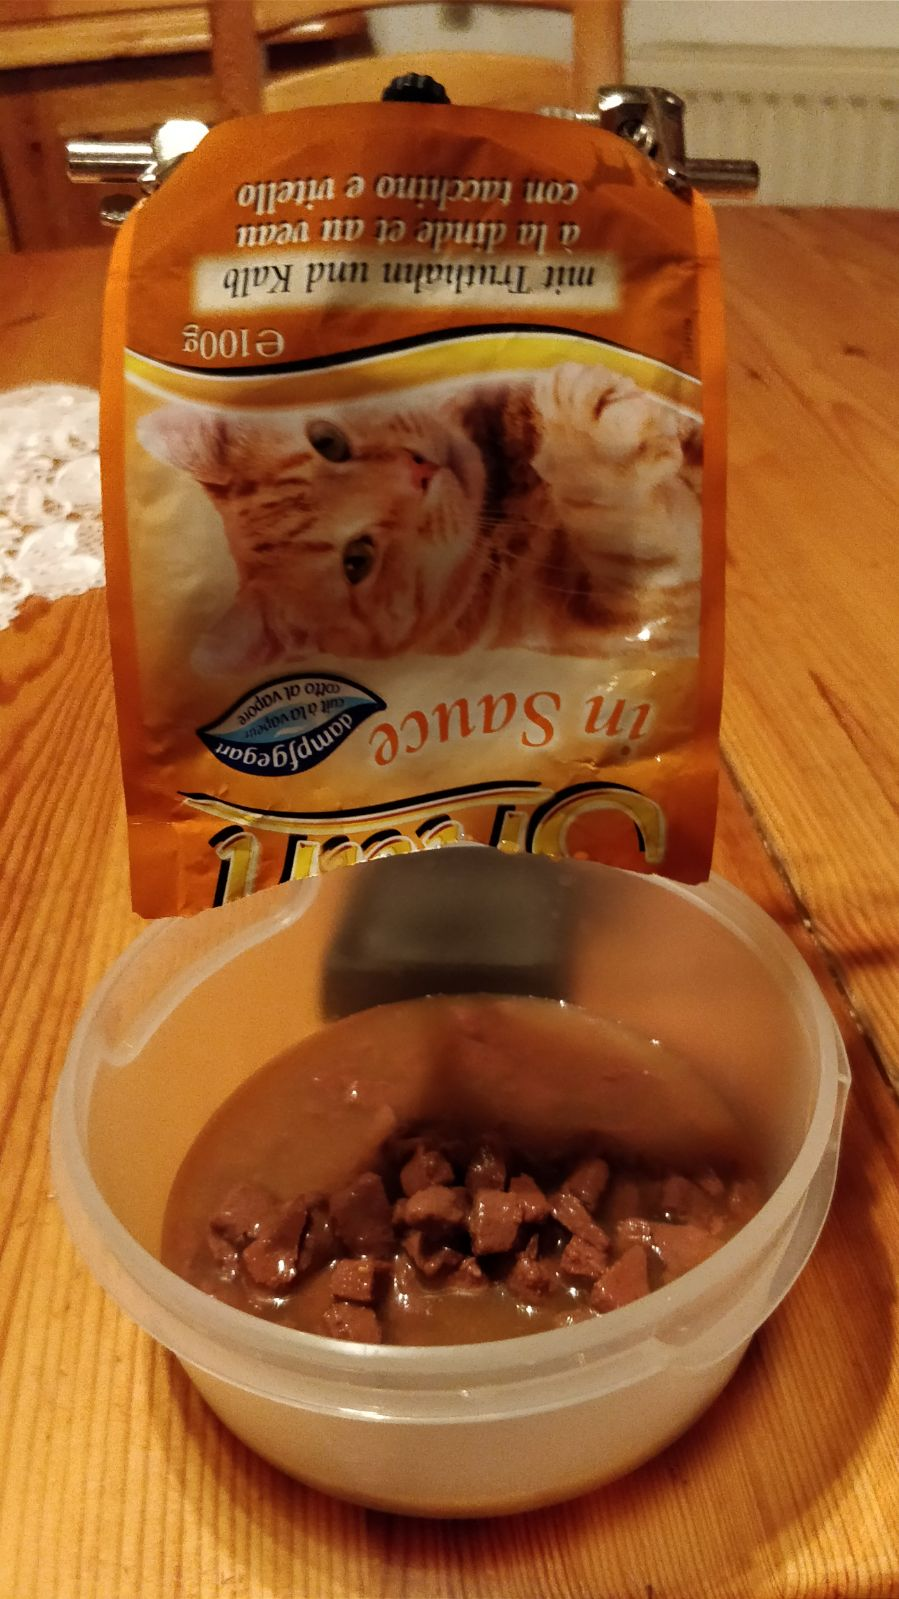
\includegraphics[width=\linewidth]{Bilder/Fuetterungsexperiment/Fuetterungs_Ende}  
      \caption{Fütterungs Ende}
     \label{Fütterungs_Ende}
   \end{minipage}
\end{figure}

In der Abbildung: \ref{Fütterungs_Ende} sieht man das nach 10 Minuten der Inhalte ganz in der Futterschüssel ist, dennoch Tropft es nach.
\newpage
\subsection{Schneideversuch 1.Art der 1.Variante}

Schnitt anhand einer praxischen Anwendung dargestellt. Der Beutel wird mithilfe einer Papierschneidemaschine geschnitten. Siehe Abbildungen: \ref{Einlegen}, \ref{Anfangsschnitt}, \ref{Endschnitt}

\begin{figure}[H]
   \begin{minipage}[hbt]{.3\linewidth} % [b] => Ausrichtung an \caption
      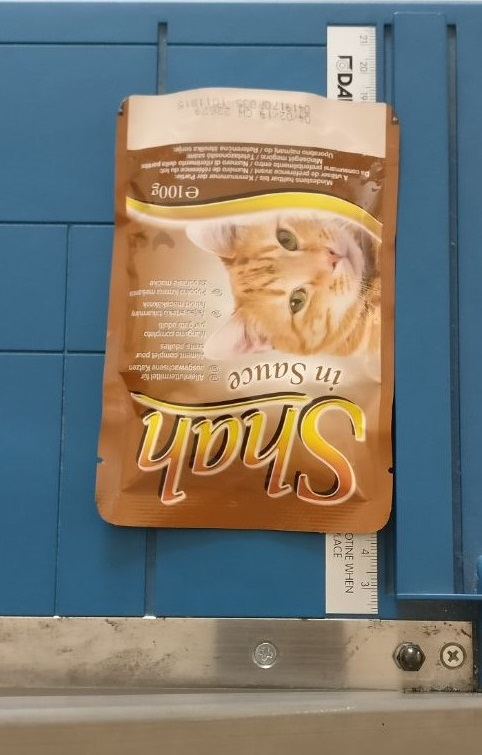
\includegraphics[width=\linewidth]{Bilder/Schneideversuch_1.Art/Einlegen}
      \caption{Einlegen}
      \label{Einlegen} 
   \end{minipage}
   \hspace{.2\linewidth}% Abstand zwischen Bilder
   \begin{minipage}[hbt]{.5\linewidth} % [b] => Ausrichtung an \caption
      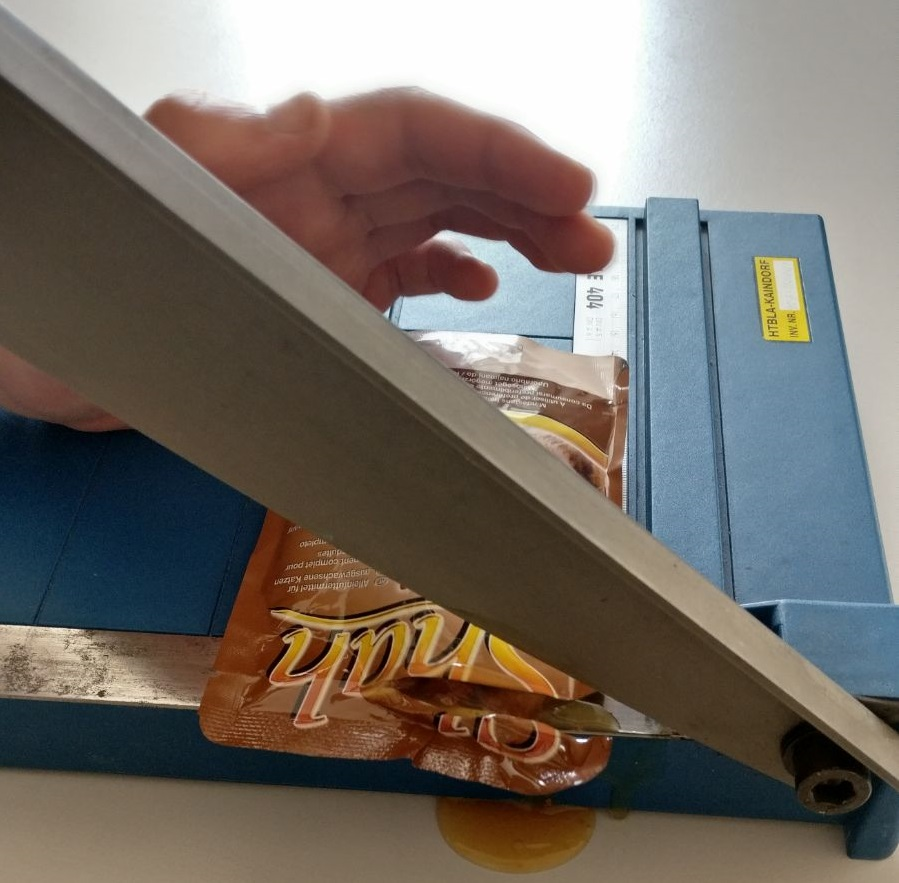
\includegraphics[width=\linewidth]{Bilder/Schneideversuch_1.Art/Anfangsschnitt}
      \caption{Anfangsschnitt}
      \label{Anfangsschnitt} 
   \end{minipage}
\end{figure}

\begin{figure}[H]
\begin{center}
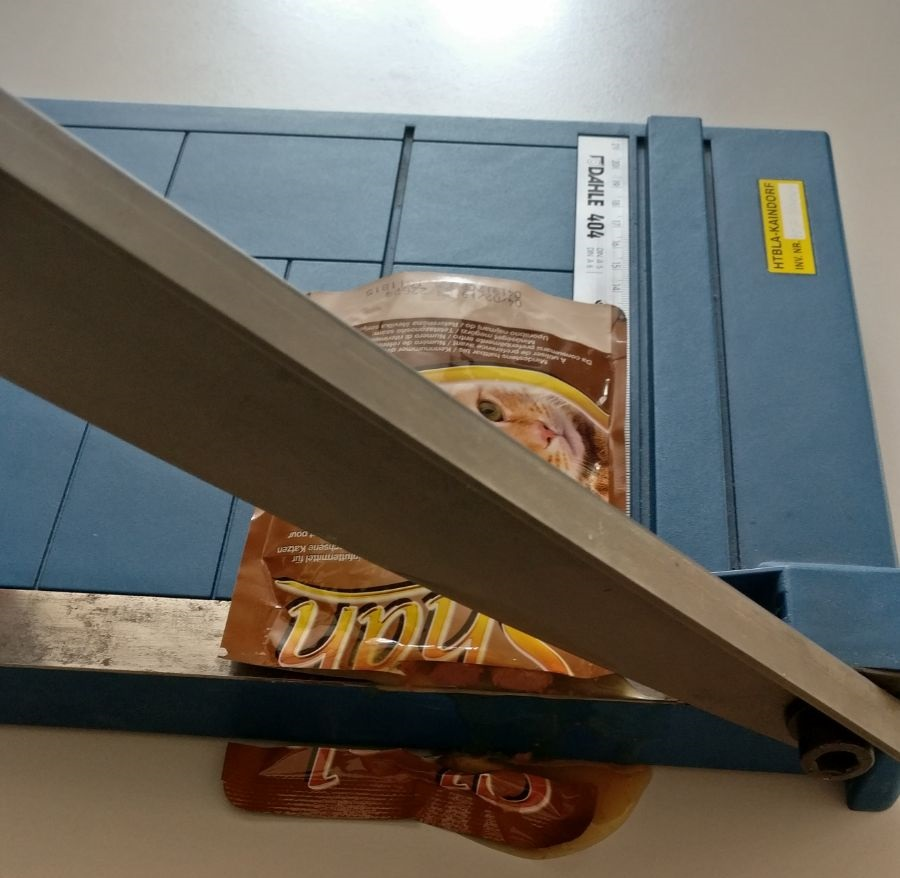
\includegraphics[width=7cm]{Bilder/Schneideversuch_1.Art/Endschnitt}
\caption{Endschnitt}
\label{Endschnitt} 
\end{center}
\end{figure}
\newpage
\subsection{Schneideversuch 2.Art der 1.Variante}

Mit einem Metallwerkzeug mit Wellenschliffartiger Kante wird der Futterbeutel entlang der Oberseite aufgeschnitten. Um die Packung vollständig geöffnet zu haben, mussten mehrere Schnitte verwendet werden. Siehe Abbildung: \ref{Schneidemittel}

\begin{figure}[H]
   \begin{minipage}[hbt]{.3\linewidth} % [b] => Ausrichtung an \caption
      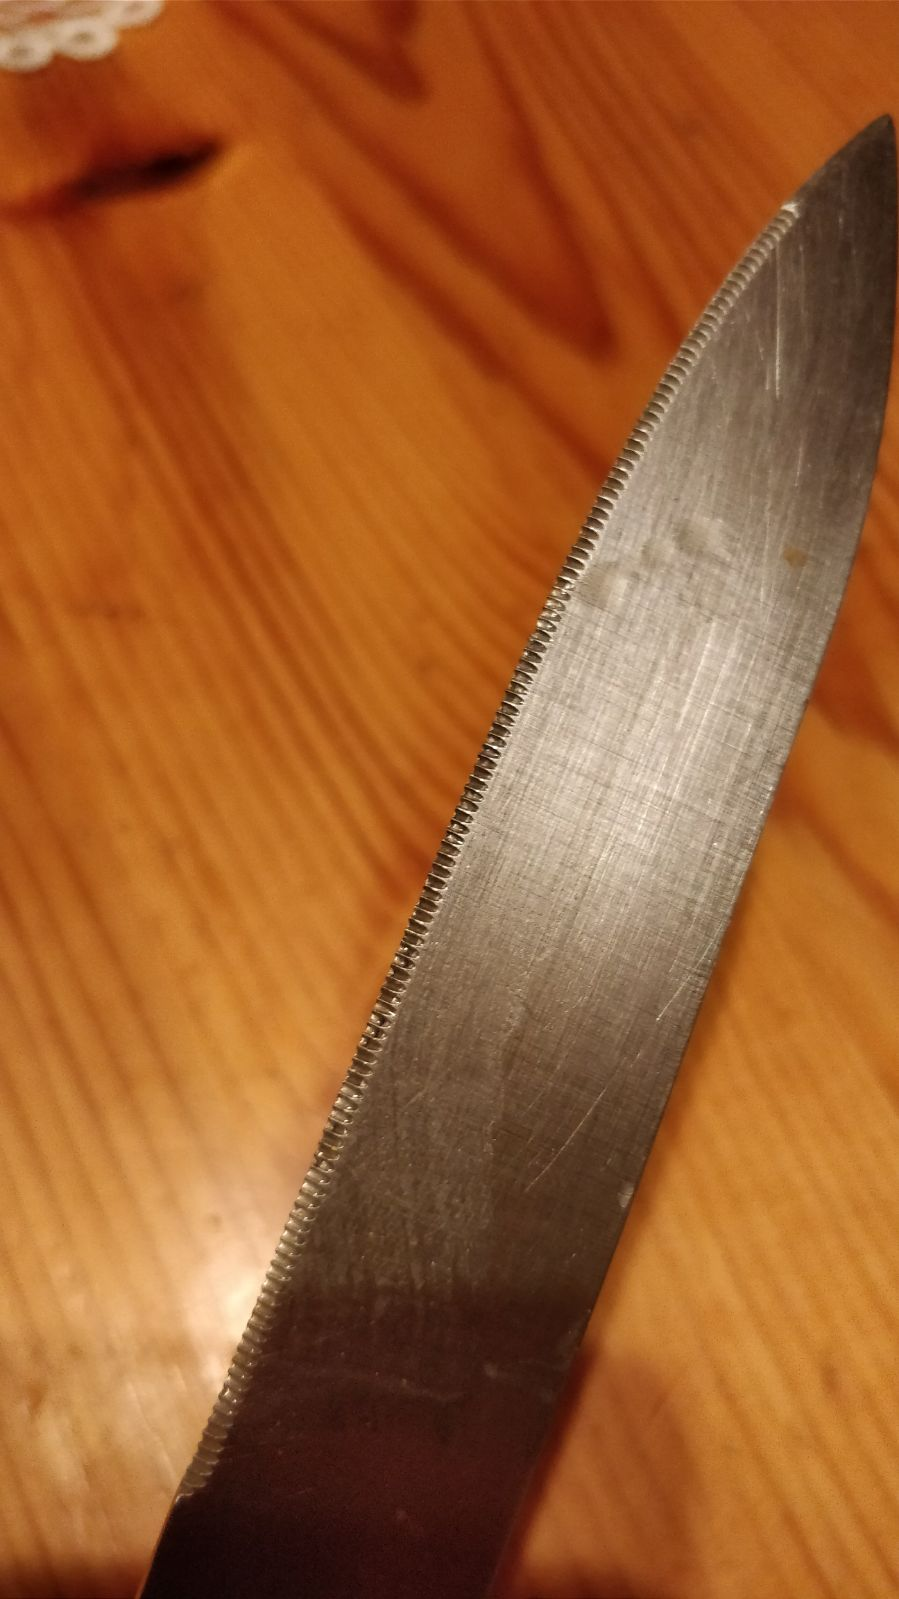
\includegraphics[width=\linewidth]{Bilder/Schneideversuch_2.Art/Schneidemittel}
      \caption{Schneidemittel}
      \label{Schneidemittel} 
   \end{minipage}
   \hspace{.4\linewidth}% Abstand zwischen Bilder
   \begin{minipage}[hbt]{.3\linewidth} % [b] => Ausrichtung an \caption
      
\includegraphics[width=\linewidth]{Bilder/Schneideversuch_2.Art/Anfangsschnitt}
      \caption{Anfangsschnitt 2.Art}
      \label{Nach 3 Schnitten}
   \end{minipage}
\end{figure}

In der Abbildung: \ref{Nach 3 Schnitten} erkennt man wie offen die Packung nach 3 Schnitten ist.

\begin{figure}[H]
   \begin{minipage}[hbt]{.4\linewidth} % [b] => Ausrichtung an \caption
      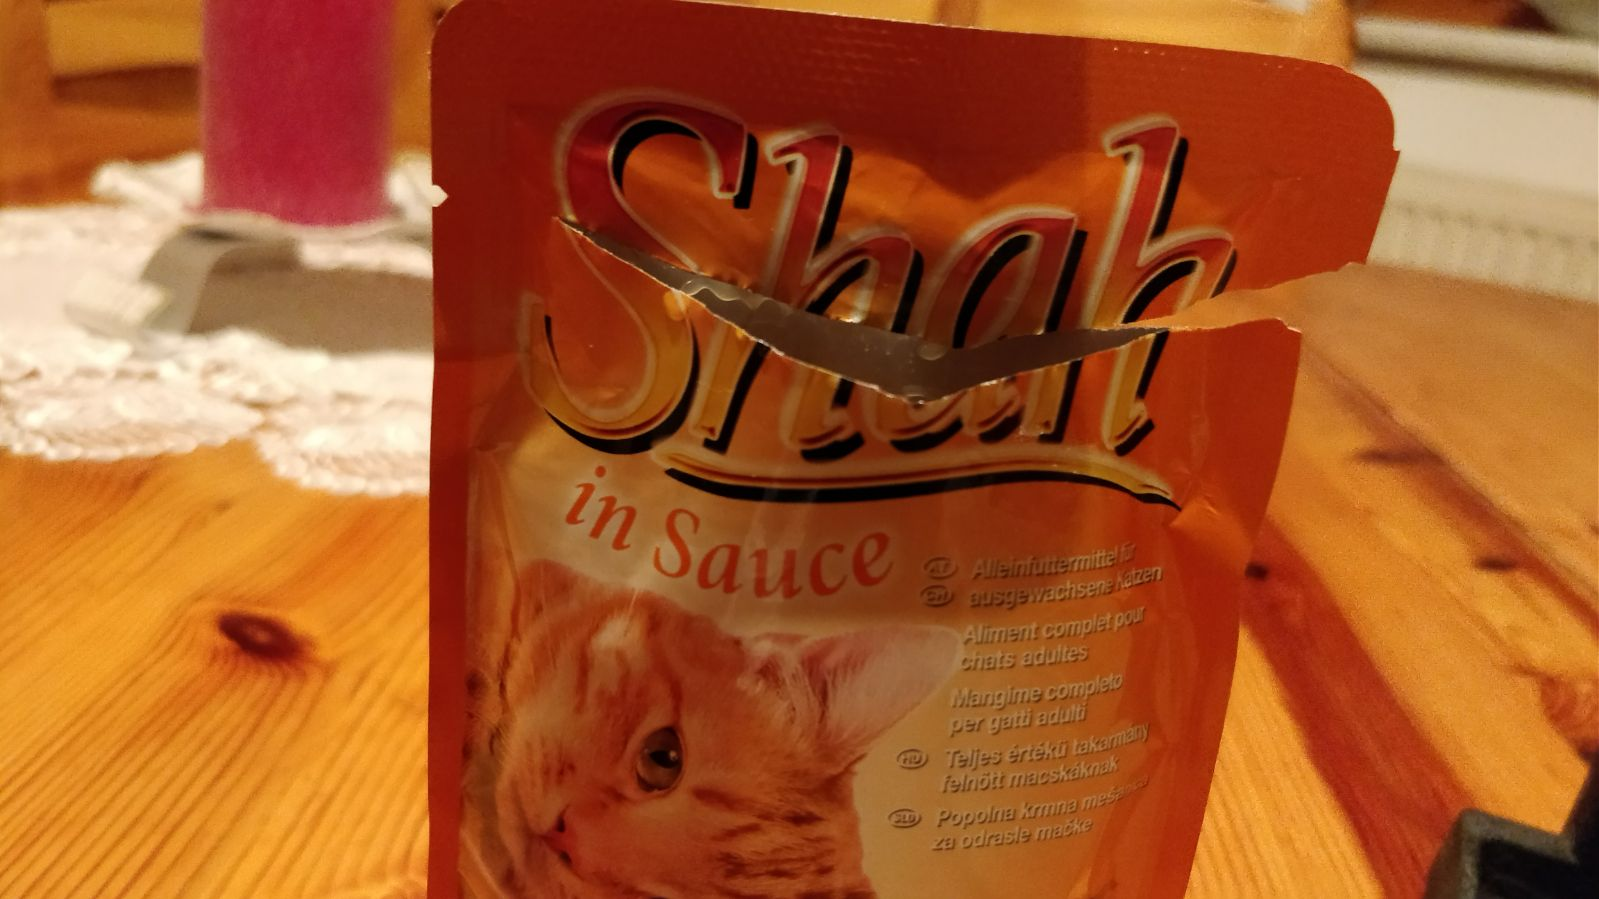
\includegraphics[width=\linewidth]{Bilder/Schneideversuch_2.Art/Mittelschnitt}
      \caption{Mittelschnitt 2.Art}
      \label{Nach 6 Schnitten}
   \end{minipage}
   \hspace{.2\linewidth}% Abstand zwischen Bilder
   \begin{minipage}[hbt]{.4\linewidth} % [b] => Ausrichtung an \caption
      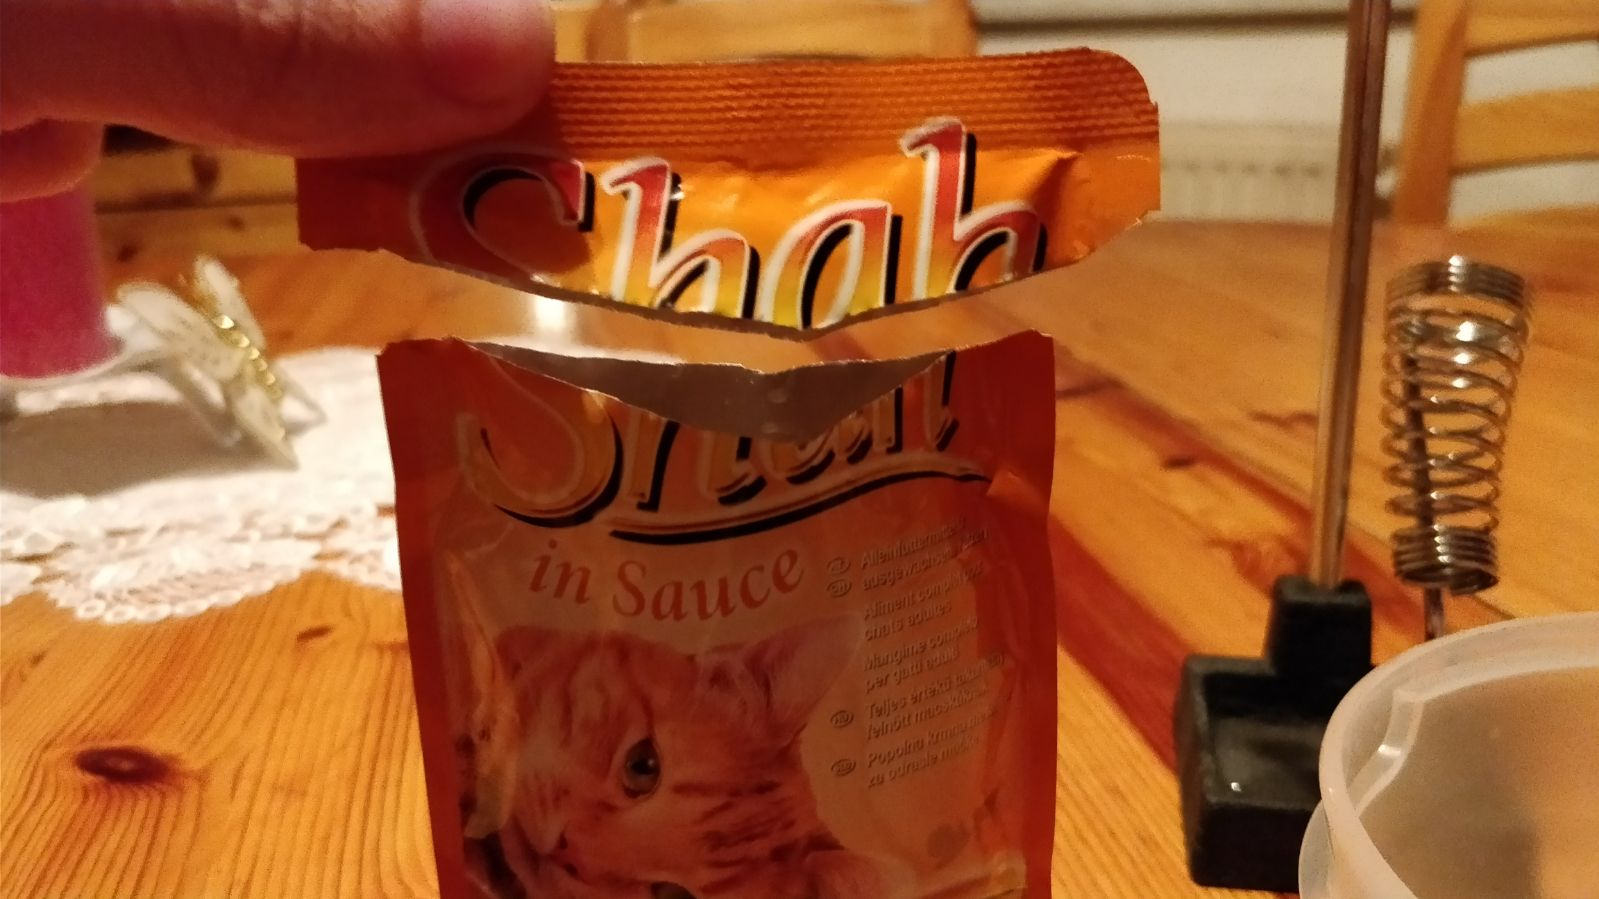
\includegraphics[width=\linewidth]{Bilder/Schneideversuch_2.Art/Endschnitt}
      \caption{Endschnitt 2.Art}
      \label{Nach 9 Schnitten}
   \end{minipage}
\end{figure}
In der Abbildung: \ref{Nach 6 Schnitten} erkennt man wie offen die Packung nach 6 Schnitten ist.\\

In der Abbildung: \ref{Nach 9 Schnitten} wurde die Packung nach 9 Schnitten vollständig geöffnet.

\section{Vergleich der Varianten}
\subsection{Klemmen}
\subsubsection{Einfache Klemme}

\begin{wrapfigure}{r}{0.5\textwidth}
\vspace{-20pt}
  \begin{center}
    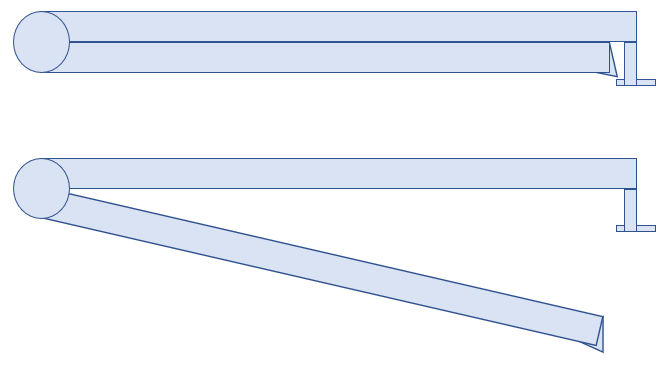
\includegraphics[width=0.32\textwidth]{Bilder/Powerpoint/Einfach_Klemme}
  \end{center}
  \caption{Einfache Klemme}
  \label{Einfache Klemme}
  \vspace{-30pt}
\end{wrapfigure}

Die einfach Klemme ist für gewöhnliche Verpackungen gut zu nutzen jedoch ist sie für unsere Variante nicht zu gebrauchen, dadurch Kunstoff nicht so stabil wie Metall ist drück sie die Packung an manchen Stellen zu wenig zusammen und an diesen Stellen kann Flüssigkeit austreten. Außerdem hält sie bei Zugbelastung nur wenig stand. Siehe Abbildung: \ref{Einfache Klemme}

\subsubsection{Hebel Klemme} 

\begin{wrapfigure}{r}{0.5\textwidth}
\vspace{-30pt}
  \begin{center}
    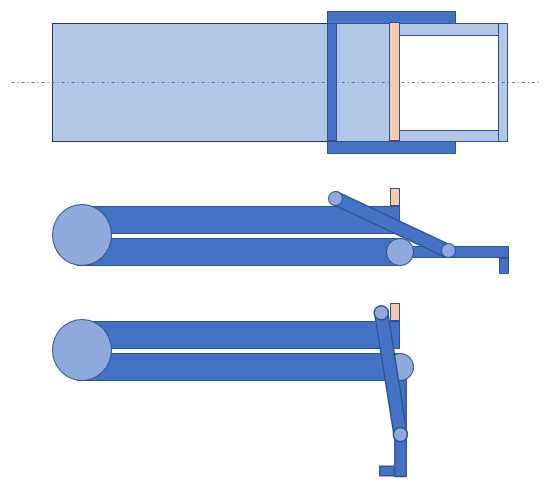
\includegraphics[width=0.32\textwidth]{Bilder/Powerpoint/Hebel_Klemme}
  \end{center}
  \caption{Hebel Klemme}
  \label{Hebel Klemme}
  \vspace{-65pt}
\end{wrapfigure}

Die Hebel Klemme ist für diese Diplomarbeit die bevorzugte Methode sie kann viel Druck auf die Packung ausüben sodass keine Flüssigkeit entrinnen kann. Außerdem lässt sich durch den Hebel mit wenig Kraft die Klemme öffnen. Weiters können die Klemmen auf einer Stange aufgesammelt werden und liegen nicht an unerwünschten Positionen an denen man nicht herankommt. Siehe Abbildung:    
 \ref{Hebel Klemme}
 \vspace{40pt}


\subsubsection{Gummiband Klemme}
 
\begin{wrapfigure}{r}{0.5\textwidth}
\vspace{-40pt}
  \begin{center}
    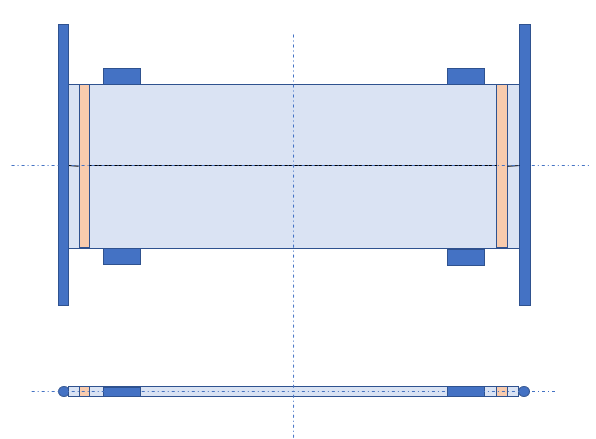
\includegraphics[width=0.30\textwidth]{Bilder/Powerpoint/Gummiband_Klemme}
  \end{center}
  \caption{Gummiband Klemme}
  \label{Gummiband Klemme}
  \vspace{-20pt}
\end{wrapfigure}

Die Gummiband Klemme hat eine starke Klemmkraft, dies Schützt vor dem Aufplatzen der Verpackung. Das Problem dieser Variante ist das das Gummiband spröder werden kann und irgendwann reißen, also ein hoher Verschleiß. Die Klemmen kann man auch nicht kontrolliert sammeln und somit sind sie schwerer zugänglich.

\subsection{Futterschüsseln}

\subsubsection{Drehfutterplatte}

\begin{wrapfigure}{r}{0.5\textwidth}
\vspace{-40pt}
  \begin{center}
    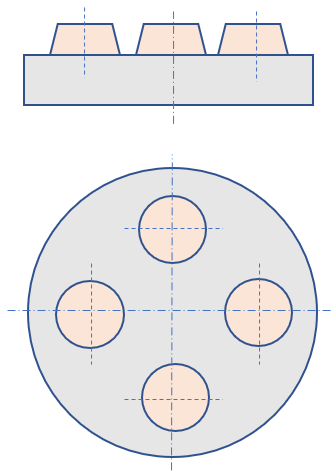
\includegraphics[width=0.25\textwidth]{Bilder/Powerpoint/Drehplatte}
  \end{center}
  \caption{Drehplatte}
  \label{Drehplatte}
  \vspace{-20pt}
\end{wrapfigure}

Die Drehplatte besteht aus fünf Schüsseln man kann pro Schüssel die Katze 2-mal am Tag füttern abends und morgens. Dadurch hat die Katze jeden Tag einen neue Schüssel und falls sie nicht frisst muss sie nicht Hunger leiden. Auf einer Welle wird eine Platte befestigt 
darin werden fünf Löcher geschnitten und die Schüssel hinein gelegt. Die Drehplatte wird mit einen Schneckengewinde in die gewünschten Position gebracht. Siehe Abbildung:  	
 \ref{Drehplatte} \vspace{+80pt}
 

\subsubsection{Futterplatte Zylinder}

\begin{wrapfigure}{}{0.5\textwidth}
\vspace{-50pt}
  \begin{center}
    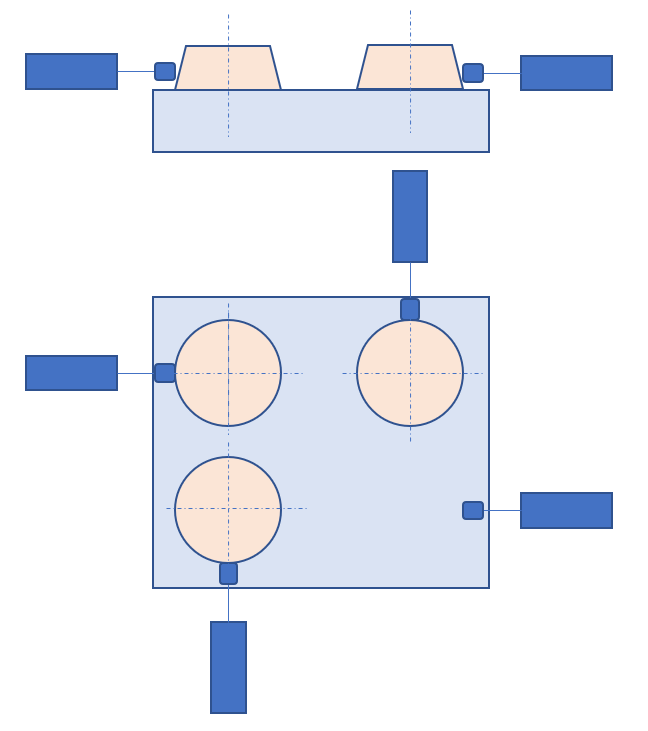
\includegraphics[width=0.32\textwidth]{Bilder/Powerpoint/Platte_Zylinder}
  \end{center}
  \caption{Platte Zylinder}
  \label{Platte Zylinder}
  \vspace{-20pt}
\end{wrapfigure}

Die Futterplatte mit Zylinder ist die umständlichste Variante. Es ist eine viereckige Platte auf der Schienen für das schieben der Futterschüsseln platziert sind. Diese werden von Magnetzylindern angeschoben. Der Nachteil hierbei ist, man benötigt viele Bauteile und alle Zylinder müssen zugleich arbeiten um die Futterschüssel zur richtigen Position zu führen. Siehe Abbildung: \ref{Platte Zylinder} 



\newpage
\subsubsection{Platte mit einer Schüssel}

\begin{wrapfigure}{r}{0.5\textwidth}
\vspace{-40pt}
  \begin{center}
    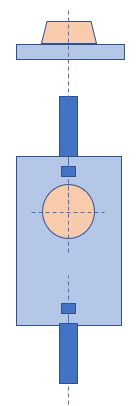
\includegraphics[width=0.17\textwidth]{Bilder/Powerpoint/Einschuessel_platte}
  \end{center}
  \caption{Einschüsselplatte}
  \label{Schüssel Eins}
  \vspace{-20pt}
\end{wrapfigure}

Die Platte mit nur einer Schüssel ist leicht zu realisieren da sie nur wenige Bauteile benötigt. Das wäre zum Einem die Platte auf der die Futterschüssel mit einer Schiene darauf platziert ist. Sowohl als auch die zwei Magnetzylinder die die Futterschüssel in die Anfangs und Endposition bringt. Jedoch ein großer Nachteil weswegen diese Methode nicht in Frage kommt ist, wenn die Katze nach dem Füttern nicht frisst dann bleibt der Inhalt in der Schale und trocknet ein oder es kommt Ungeziefer hinein. Das hat zu Folge das die Schüssel jeden Tag befüllt wird und übergeht. Siehe Abbildung: \ref{Schüssel Eins} 



\subsection{Futtermagazine}

\subsubsection{Futtermagazin Horizontal}

\begin{wrapfigure}{r}{0.5\textwidth}
\vspace{-40pt}
  \begin{center}
    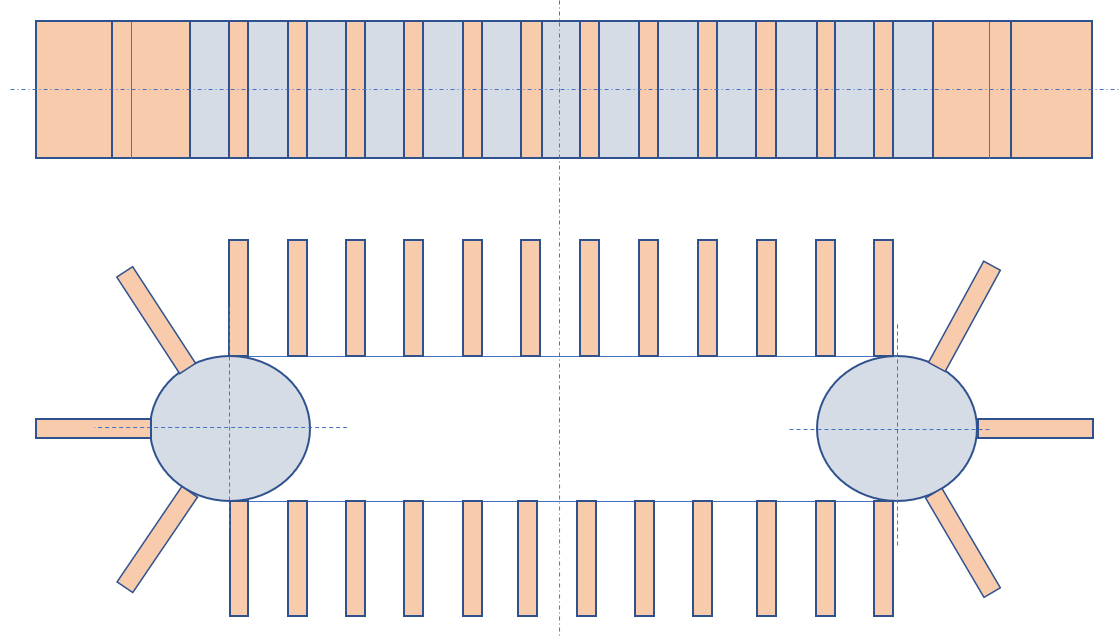
\includegraphics[width=0.30\textwidth]{Bilder/Powerpoint/Futtermagazin_horizontal}
  \end{center}
  \caption{Futtermagazin Horizontal}
  \label{Magazin Horizontal}
  \vspace{-10pt}
\end{wrapfigure} 

Das Futtermagazin Horizontal wäre für die erste Variante optimal. Da man den gewünschten Vorrat an Futterpackungen in die abgetrennten Räume platziert. Somit ist es einfach die gewünschte Position anzufahren und mit einen Greifer in die Schneideposition zu bringen. Der Aufbau ist wie ein Förderband, zwei Räder, ein Band mit oben platzierten Trennwänden und ein Motor der dieses Futtermagazin in Bewegung bringt. Zu beachten wäre wie die Futterpackungen ins Magazin eingelegt werden, nämlich mit der dünneren Fläche mit der Einkerbung die der Hersteller angegeben hat. Siehe Abbildung: \ref{Magazin Horizontal}
\newpage
\subsubsection{Futtermagazin Vertikal}

\begin{wrapfigure}{r}{0.5\textwidth}
\vspace{-40pt}
  \begin{center}
    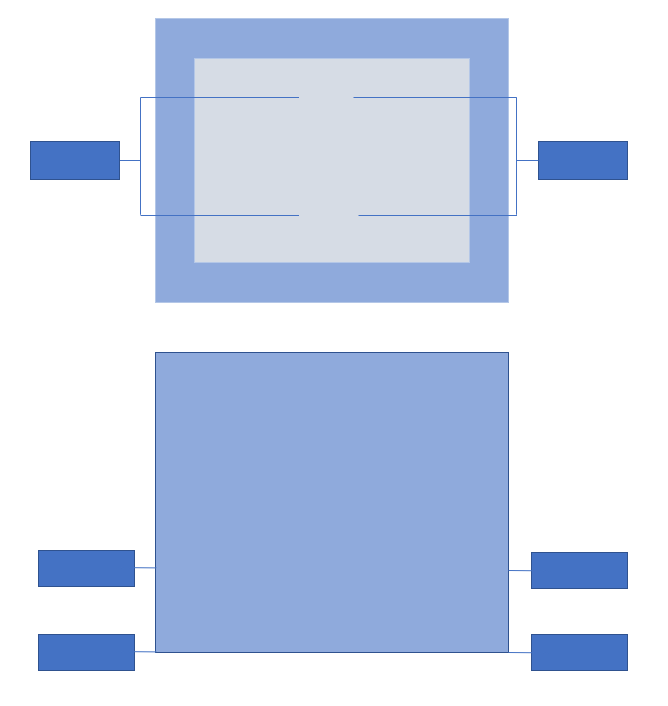
\includegraphics[width=0.26\textwidth]{Bilder/Powerpoint/Futtermagazin_vertikal}
  \end{center}
  \caption{Futtermagazin Vertikal}
  \label{Magazin Vertikal}
  \vspace{-10pt}
\end{wrapfigure}

Das Futtermagazin Vertikal ist ein rechteckiges Gehäuse an denen 4 Magnetzylinder platziert werden. In dieser Box kommen die 10 Futterpackungen. Der Ablauf funktioniert in einer gewissen Reihenfolge. Zuerst öffnet sich der erste linke Magnetzylinder danach der gegenüberliegende zweite Magnetzylinder. Daraufhin gelangt die erste Futterpackung auf die unteren Zylinder. Nach diesem Schritt schließen sich die beiden Magnetzylinder wieder, damit die anderen Packungen nach den öffnen der unteren Magnetzylinder nicht durch die Maschine fallen. Daraufhin wenn der Fütterungsbefehl kommt öffnen sich die unteren Zylinder und die Packung gleitet über ein Blech zur Schnittfläche. Der große Nachteil dieser Methode ist das immer wieder Fehler auftreten können. Die Futterpackung kann falsch an der Schneidfläche ankommen bzw. sich an einem bestimmten Ort verkeilen. Siehe Abbildung: \ref{Magazin Vertikal}

\section{Konstruktion der Wahlvariante und Details}

\subsection{Drehplatte}
\subsection{Förderband}

\subsection{Walze}
\section{Berechnung und Dimensionierung}
\section{Simulation}
\section{Bedienung und Wartung}
\section{Selbstkritische Analyse und Ausblick}

